%============================ MAIN DOCUMENT ================================
% define document class
\PassOptionsToPackage{table}{xcolor}
\documentclass[
  a4paper,
  BCOR=15mm,            % Binding correction
  twoside=false,
% openright,
%  headings=openright,
  bibliography=totoc,   % If enabled add bibliography to TOC
  listof=totoc,         % If enabled add lists to TOC
  monolingual,
% bilingual,
% invert-title,
]{bfhthesis}

\LoadBFHModule{listings,terminal,boxes}
%---------------------------------------------------------------------------
% Documents paths
%---------------------------------------------------------------------------
\makeatletter
\def\input@path{{content/}}
%or: \def\input@path{{/path/to/folder/}{/path/to/other/folder/}}
\makeatother
%-----------------  Base packages     --------------------------------------
% Include Packages
\usepackage[french,ngerman,main=english]{babel}  % https://www.namsu.de/Extra/pakete/Babel.html

\usepackage{amsmath}          % various features to facilitate writing math formulas
\usepackage{amsthm}           % enhanced version of latex's newtheorem
\usepackage{amsfonts}         % set of miscellaneous TeX fonts that augment the standard CM
\usepackage{amssymb}          % mathematical special characters

\usepackage{siunitx}

\usepackage{graphicx}         % integration of images
\usepackage{float}            % floating objects

\usepackage{caption}          % for captions of figures and tables
\usepackage{subcaption}       % for subcaptions in subfigures
\usepackage{cite}             % use bibtex
\usepackage{wrapfig}

\usepackage{exscale}          % mathematical size corresponds to textsize
\usepackage{multirow}         % multirow emables combining rows in tables
\usepackage{multicol}

\usepackage{longtable}

\usepackage{parskip}

%---------------------------------------------------------------------------
% Graphics paths
%---------------------------------------------------------------------------
\graphicspath{{pictures/}{figures/}}
%---------------------------------------------------------------------------
% Blind text -> for dummy text
%---------------------------------------------------------------------------
\usepackage{blindtext}    
\usepackage{letltxmacro}   
\LetLtxMacro{\blindtextblindtext}{\blindtext}

\RenewDocumentCommand{\blindtext}{O{\value{blindtext}}}{
	\begingroup\color{BFH-Gray}\blindtextblindtext[#1]\endgroup
}
%---------------------------------------------------------------------------
% Glossary Package
%---------------------------------------------------------------------------
% the glossaries package uses makeindex
% if you use TeXnicCenter do the following steps:
%  - Goto "Ausgabeprofile definieren" (ctrl + F7)
%  - Select the profile "LaTeX => PDF"
%  - Add in register "Nachbearbeitung" a new "Postprozessoren" point named Glossar
%  - Select makeindex.exe in the field "Anwendung" ( ..\MiKTeX x.x\miktex\bin\makeindex.exe )
%  - Add this [ -s "%tm.ist" -t "%tmx.glg" -o "%tm.gls" "%tm.glo" ] in the field "Argumente"
%
% for futher informations go to http://ewus.de/tipp-1029.html
%---------------------------------------------------------------------------
\usepackage[nonumberlist]{glossaries-extra}
\makeglossaries
\newglossaryentry{agile}{
  name={Agile},
  description={A set of software development methods based on iterative development, where requirements and solutions evolve.},
  plural=agiles
}

\newglossaryentry{Kanban}{
  name={Kanban},
  description={A method for managing tasks and workflows.},
  plural=Kanbans
}

\newglossaryentry{backlog}{
  name={Backlog},
  description={A list of tasks that need to be done.},
  plural=backlogs
}

 \newglossaryentry{Software stack}{
  name={Software stack},
  text={software stack},
  description={A set of software components that are used to build a software system.},
  plural=Software stacks
 }

 \newglossaryentry{Data flow}{
  name={Data flow},
  text={data flow},
  description={The flow of data between components in a system.},
  plural=Data flows
 }

 \newglossaryentry{functional requirements}{
  name={Functional requirements},
  text={Functional requirements},
  description={Requirements that define the functionality of a system.},
  plural=functional requirements
 }

\newglossaryentry{non-functional requirements}{
  name={non-functional requirements},
  text={non-functional requirements},
  description={Requirements that are not necessarily functional.},
  plural=non-functional requirements
}

\newglossaryentry{proprietary}{
  name={Proprietary},
  text={proprietary},
  description={A term used to describe software that is not open source and is owned by somebody.},
  plural=proprietary
}

\newglossaryentry{modular}{
  name={Modular},
  text={modular},
  description={Something that is made up of multiple parts that can be replaced or removed.},
  plural=modular
}

\newglossaryentry{sensors}{
  name={Sensors},
  text={sensors},
  description={A device that detects a physical phenomenon and converts it into a signal that can be read by a computer.},
  plural=sensors
}

\newglossaryentry{actuators}{
  name={Actuators},
  text={actuators},
  description={A device that converts a signal into a physical phenomenon.},
  plural=actuators
}

\newglossaryentry{4G}{
  name={4G},
  text={4G},
  description={A mobile communication standard that is used to transmit data over a cellular network.},
  plural=4G
}

\newglossaryentry{LTE-M}{
  name={LTE-M},
  text={LTE-M},
  description={A mobile communication standard that is used to transmit data over a cellular network.},
  plural=LTE-M
}

\newglossaryentry{ecosystem}{
  name={Ecosystem},
  text={ecosystem},
  description={Infermation technology specific definition: A set of components that work together to provide a specific functionality.},
  plural=ecosystems
}

\newglossaryentry{Open source}{
  name={Open source},
  text={open source},
  description={A term used to describe software that is free to use and modify.},
  plural=open source
}

\newglossaryentry{Apiary}{
  name={Apiary},
  text={apiary},
  description={A place where bees are kept.},
  plural=Apiary
}

\newglossaryentry{amplifier}{
  name={Amplifier},
  text={amplifier},
  description={A device that increases the power of a signal.},
  plural=amplifiers
}

\newglossaryentry{Brood chamber}{
  name={Brood chamber},
  text={brood chamber},
  description={A chamber in a beehive where the queen lays eggs.},
  plural=brood chambers
}

\newglossaryentry{GSM}{
  name={GSM},
  text={GSM},
  description={A mobile communication standard that is used to transmit data over a cellular network.},
  plural=GSM
}

\newglossaryentry{GPRS}{
  name={GPRS},
  text={GPRS},
  description={A mobile communication standard that is used to transmit data over a cellular network.},
  plural=GPRS
}

\newglossaryentry{SIM}{
  name={SIM},
  text={SIM},
  description={A SIM card (Subscriber Identity Module) is used to authenticate a user in a mobile network},
  plural=SIM
}

\newglossaryentry{DC}{
  name={DC},
  text={DC},
  description={Direct electrical current.},
  plural=DC
}

\newglossaryentry{Arduino IDE}{
  name={Arduino IDE},
  text={Arduino IDE},
  description={A development environment used to develop for the Arduino plattform.}
  plural={Arduino IDE}
}

\newglossaryentry{Sensor Block}{
  name={Sensor Block},
  text={Sensor Block},
  description={A closed system consisting of multiple sensors and/or actuators.},
  plural=Sensor Blocks
}

\newglossaryentry{Data Broker}{
  name={Data Broker},
  text={Data Broker},
  description={A service that manages the collection, storage, and distribution of data. MQTT in this context is a data broker.},
  plural=Data Brokers
}

\newglossaryentry{Backend}{
  name={Backend},
  text={Backend},
  description={The part of a system that is not directly accessible to the user.},
  plural=backends
}

\newglossaryentry{Database}{
  name={Database},
  text={Database},
  description={A system that stores data.},
  plural=databases
}

\newglossaryentry{User Interface}{
  name={User Interface},
  text={User Interface},
  description={The part of a system that is directly accessible to the user.},
  plural=User Interfaces
}

\newglossaryentry{Architecture}{
  name={Architecture},
  text={Architecture},
  description={The structure of a system.},
  plural=Architectures
}

\newglossaryentry{ESP32}{
  name={ESP32},
  text={ESP32},
  description={A microcontroller that is used to build IoT devices.},
  plural=ESP32
}

\newglossaryentry{Firmware}{
  name={Firmware},
  text={Firmware},
  description={The software that is installed on a microcontroller and generally doesn't get changed.},
  plural=Firmware
}

\newglossaryentry{Mosquitto}{
  name={Mosquitto},
  text={Mosquitto},
  description={A MQTT broker.},
  plural=Mosquitto
}

\newglossaryentry{MQTT}{
  name={MQTT},
  text={MQTT},
  description={A protocol that is used to communicate between devices.},
  plural=MQTT
}

\newglossaryentry{Prototype}{
  name={Prototype},
  text={Prototype},
  description={A working model of a system.},
  plural=Prototypes
}

\newglossaryentry{Docker}{
  name={Docker},
  text={Docker},
  description={A tool that is used to create and manage software containers.},
  plural=Docker
}

\newglossaryentry{TLS}{
  name={TLS},
  text={TLS},
  description={A protocol that is used to encrypt data.},
  plural=TLS
}

\newglossaryentry{HTTP}{
  name={HTTP},
  text={HTTP},
  description={A protocol that is used to transfer data over the internet.},
  plural=HTTP
}

\newglossaryentry{API}{
  name={API},
  text={API},
  description={An interface that is used to interact with a system.},
  plural=API
}

\newglossaryentry{Middleware}{
  name={Middleware},
  text={middleware},
  description={A software layer that is used to connect different systems.},
  plural=Middleware
}

\newglossaryentry{Endpoint}{
  name={Endpoint},
  text={endpoints},
  description={A point of interaction with a system.},
  plural=Endpoints
}

\newglossaryentry{ORM}{
  name={ORM},
  text={ORM},
  description={A system that is used to manage the relation between data in a database and the data in a programming language.},
  plural=ORM
}

\newglossaryentry{Reverse Proxy}{
  name={Reverse Proxy},
  text={reverse proxy},
  description={A system that is used to forward requests to a backend.},
  plural=Reverse Proxy
}

\newglossaryentry{Port}{
  name={Port},
  text={port},
  description={A number that is used to identify a specific service.},
  plural=Ports
}

\newglossaryentry{Timestamp}{
  name={Timestamp},
  text={timestamp},
  description={A number that is used to identify a specific point in time.},
  plural=Timestamps
}

\newglossaryentry{IOT}{
  name={IOT},
  text={IOT},
  description={The Internet of Things.},
  plural=IOT
}

\newglossaryentry{Off-Grid}{
  name={Off-Grid},
  text={off-grid},
  description={A system that is not connected to the electrical grid.},
  plural=Off-Grid
}

\newglossaryentry{Microcontroller}{
  name={Microcontroller},
  text={microcontroller},
  description={A small computer that is used to control devices.},
  plural=Microcontrollers
}

\newglossaryentry{CSV}{
  name={CSV},
  text={CSV},
  description={A file format that is used to store data.},
  plural=CSV
}

\newglossaryentry{Data sheet}{
  name={Data sheet},
  text={data sheet},
  description={A document that contains information about a specific component.},
  plural=Data sheets
}

\newglossaryentry{18650}{
  name={18650},
  text={18650},
  description={A common type of battery.},
  plural=18650
}

\newglossaryentry{Client}{
  name={Client},
  text={client},
  description={A user-facing system that is used to interact with a server.},
  plural=clients
}

\newglossaryentry{Proof of Concept}{
  name={Proof of Concept},
  text={proof of concept},
  description={A working model of a system that is used to demonstrate the feasibility of a system.},
  plural=Proof of Concepts
}

\newglossaryentry{Off the shelf}{
  name={Off the shelf},
  text={off the shelf},
  description={A system that is ready to use.},
  plural=Off the shelf
}
%---------------------------------------------------------------------------
% Makeindex Package
%---------------------------------------------------------------------------
\usepackage{makeidx}
\makeindex
%\usepackage{imakeidx}          % To produce index
%\makeindex[columns=2,intoc]    % Index-Initialisation
%\makeindex[columns=3,columnseprule,columnsep,intoc]
%---------------------------------------------------------------------------
% Hyperref Package (Create links in a pdf)
%---------------------------------------------------------------------------
\usepackage[
	,bookmarks
	,plainpages=false
	,pdfpagelabels
        ,pdfusetitle
	,backref = {false}          % No index backreference
	,colorlinks = {true}        % Color links in a PDF
	,hypertexnames = {true}     % no failures "same page(i)"
	,bookmarksopen = {true}     % opens the bar on the left side
	,bookmarksopenlevel = {0}   % depth of opened bookmarks
	,linkcolor=.
	,filecolor=.
	,urlcolor=.
	,citecolor=.
]{hyperref}
%---------------------------------------------------------------------------

%% %% Customize Footer and Headers in Document
%% \KOMAoptions{headsepline,plainheadsepline,footsepline,plainfootsepline}%
%% \setkomafont{headsepline}{\color{BFH-DarkBlue}}% BFH-DarkBlue required bfhcolors
%% \setkomafont{footsepline}{\color{BFH-DarkBlue}}%
%% \lehead*{lehead} % the * character does replace the header on the first chapter page as well
%% \cehead*{cehead}
%% \rehead*{rehead}
%% \lohead*{lohead}
%% \cohead*{cohead}
%% \rohead*{rohead}

%% \lefoot*{lefoot}
%% \cefoot*{cefoot}
%% \refoot*{refoot}
%% \lofoot*{lofoot}
%% \cofoot*{cofoot}
%% \rofoot*{rofoot}
%---------------------------------------------------------------------------
\begin{document}

%------------ START FRONT PART ------------
\frontmatter

\title{HiveTracker}
\subtitle{A low cost IOT sensor station for beekeepers}
\author{Nicolo Lüscher}
\institution{Bern University of Applied Sciences}
\department{Technik und Informatik}
\institute{Computer Sciences}
\version{1.0}
\titlegraphic*{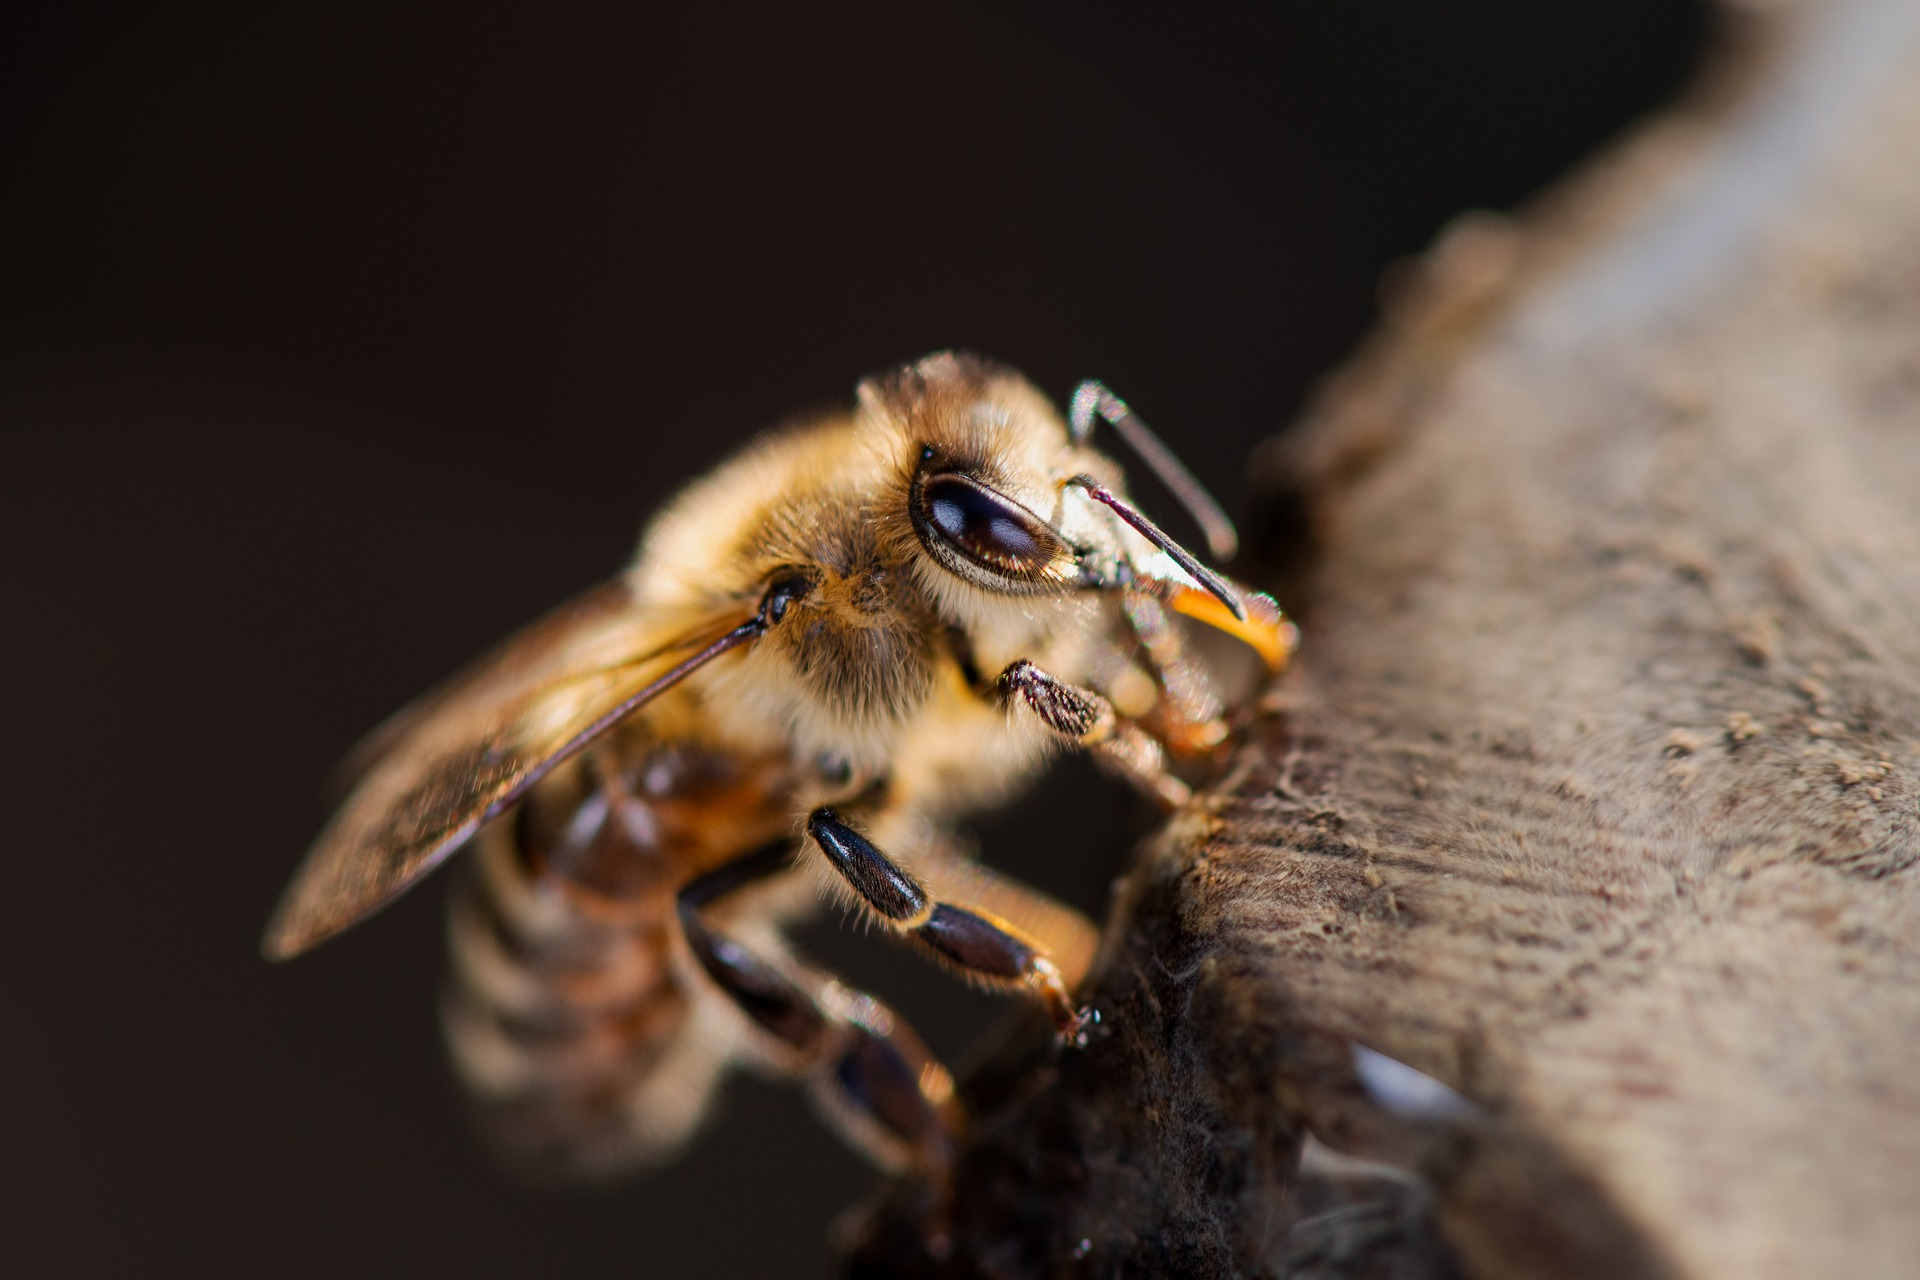
\includegraphics{bee}}
\advisor{Prof. Dr. Andreas Danuser}
\degreeprogram{Bachelor of Science in Computer Science}
\setupSignature{
	Nicolo Lüscher={\includegraphics[width=.5\linewidth]{signature_nicolo_lüscher.png}}
}


%----------------  BFH tile page   -----------------------------------------
\maketitle
\section*{Abstract}

Abstract

%------------ TABLEOFCONTENTS ----------------
\tableofcontents

%------------ START MAIN PART ------------
\mainmatter

\chapter{Introduction}

\section{Motivation}
A family member of mine approached me with the request of looking into ways to monitor their beehives. They wanted to collect some basic information about their colonies like weight and temperature. This information should be made available over the internet and should be displayed in an easy-to-read format. The goal was to have an overview over the colonies and to be able to react to changes.

After listening to the request of my family member, I decided to look at the solutions that are commercially available. These are quite expensive, proprietary and not open source. Most of them also required a subscription from the manufacturer to work. I decided to look into the possibility of building my own solution. This would allow me to have a solution that is tailored to my needs and is open source.

This project was realized in the context of my Project 2 course at the Berne University of Applied Sciences.

\newpage
\section{Method}
Given that I was the only one working on this project, I decided to use a simple \gls{agile} development process. This process did not follow any classical agile methodology, but rather a simplified version of \gls{Kanban}. The process consisted of me defining a set of tasks that needed to be done. These tasks were then put into a \gls{backlog}. I then picked a task from the backlog and started working on it. Once the task was completed, I moved onto the next one. This process was repeated until the project was completed.
The tasks were grouped into a set of categories.

\subsection{Phases}

\subsubsection{Planning}
\textbf{Task: Research existing solutions}
\begin{itemize}
    \item Research existing solutions.
    \item Compare existing solutions.
    \item Analyze features of existing solutions.
\end{itemize}

\textbf{Task: Define requirements}
\begin{itemize}
    \item Define functional requirements.
    \item Define non-functional requirements.
    \item Discuss requirements with family member.
\end{itemize}

\textbf{Task: Rough Hardware Planning}
\begin{itemize}
    \item Define overall setup in regard to the functional requirements.
    \item Define components.
    \item Define communication protocols.
\end{itemize}

\textbf{Task: Specific Hardware Planning}
\begin{itemize}
    \item Define specific components.
    \item Define physical setup.
    \item Define wiring.
\end{itemize}

\newpage
\textbf{Task: Software Planning}
\begin{itemize}
    \item Define software stack.
    \item Define software architecture.
    \item Define data format.
    \item Define communication protocols.
    \item Define data flow.
    \item Define user interface.
\end{itemize}

\subsubsection{Implementation}
\textbf{Task: Build Prototype}
\begin{itemize}
    \item Procure components.
    \item Cut raw materials.
    \item Assemble prototype.
    \item Solder components.
    \item Test Components.
\end{itemize}

\textbf{Task: Server Setup}
\begin{itemize}
    \item Setup Docker environment.
    \item Setup MQTT broker.
    \item Setup PostgreSQL database.
    \item Setup NodeJS server.
    \item Integrate Express into NodeJS server.
    \item Integrate SequelizeJS into NodeJS server.
    \item Create database models.
    \item Persist MQTT messages into database.
    \item Create API routing.
    \item Create API endpoints.
\end{itemize}

\newpage
\textbf{Task: User Interface Setup}
\begin{itemize}
    \item Setup Angular environment.
    \item Integrate Tailwind CSS into Angular.
    \item Integrate ChartJS into Angular.
    \item Create basic layout.
    \item Create data service.
    \item Visualize data with ChartJS.
\end{itemize}

\subsubsection{Testing}
\textbf{Task: Test Setup}
\begin{itemize}
    \item Setup test environment.
    \item Test weight sensor.
    \item Test weight calibration.
    \item Test temperature sensor.
    \item Test power consumption.
    \item Test user interface.
    \item Test end to end communication.
\end{itemize}

\subsubsection{Documentation}
\textbf{Task: Documentation}
\begin{itemize}
    \item Setup LaTeX environment.
    \item Write documentation.
\end{itemize}
\chapter{Realization}

\section{Planning}
The first phase of the project was the planning phase. In this phase I researched existing solutions and defined the requirements for the project. I also planned the hardware and software setup for my project. This included defining the components, the software stack and the data flow.

\subsection{Requirements}
To start of this project I had to define a set of requirements that the solution should fulfill. These requirements were then used to guide the design of the solution. I sat down with my family member and discussed the functional and non-functional requirements. The functional requirements were the features that the solution should have. The non-functional requirements were the requirements that were not directly related to the functionality of the solution.

\newpage
\subsection{Functional Requirements}
\begin{itemize}
    \item The solution should be able to be deployed in any location.
    \item The solution should include its own power supply.
    \item The solution should be able to connect to the internet in a location independent manner.
    \item The solution should be able to measure the weight of the beehive.
    \item The solution should be able to measure the temperature of the beehive.
    \item The solution should publish the data it collects to the internet.
    \item The solution should save the data it collects in a persistent manner.
    \item The solution should not require any special equipment to be installed.
    \item The solution should be able to be installed in a standard beehive.
    \item The solution should be implementation independent. Meaning that the individual components can be replaced with other components that fulfill the same function.
\end{itemize}
\subsection{Non-Functional Requirements}
\begin{itemize}
    \item The solution should be as energy efficient as possible.
    \item The solution should be able to generate its own power.
    \item The solution should be resistant to the elements.
    \item The solution should be as cost-effective as possible.
    \item The solution should be simple to build.
    \item The solution should be easy to maintain.
    \item The solution should be easy to extend.
\end{itemize}

\newpage
\subsection{Current Solutions}
It was important for me that I did not reinvent the wheel and add something to the existing solutions. I therefore researched existing solutions and compared them to my requirements. I found that there are a lot of solutions for beekeepers. Most of them are either very expensive or very complex. I also found that most of the solutions are not open source. This means that the data is not accessible to the beekeeper. This is a problem because the beekeeper should be able to access the data and analyze it in the way they want to and not rely on any proprietary solutions that might not provide them with the information they need. Furthermore, most of the solutions are not modular. This means that the beekeeper is not able to add new sensors or actuators to the system. This is a problem because the beekeeper should be able to add new sensors and actuators to the system. Most of the solutions are also unreasonably expensive and bind the user to a subscription. This means that the beekeeper has to invest a lot of money into the system that doesn't have an obvious return of investment.

\newpage
\subsubsection{HiveWatch}

\begin{figure}
    \centering
    
\includegraphics[width=0.75\textwidth]{figures/hivewatch_logo.png}
    \caption{HiveWatch}
    \label{fig:hivewatch}
\end{figure}
HiveWatch is a swiss-made, all in one solution to measure the weight of a beehive. It consists of a "transmitter" that can connect up to 8 scales that are also sold by the company. This seems to be done with a proprietary connector that isn't documented very well. It uses a 4G/LTE-M connection to connect to the internet.

\begin{figure}
    \centering
    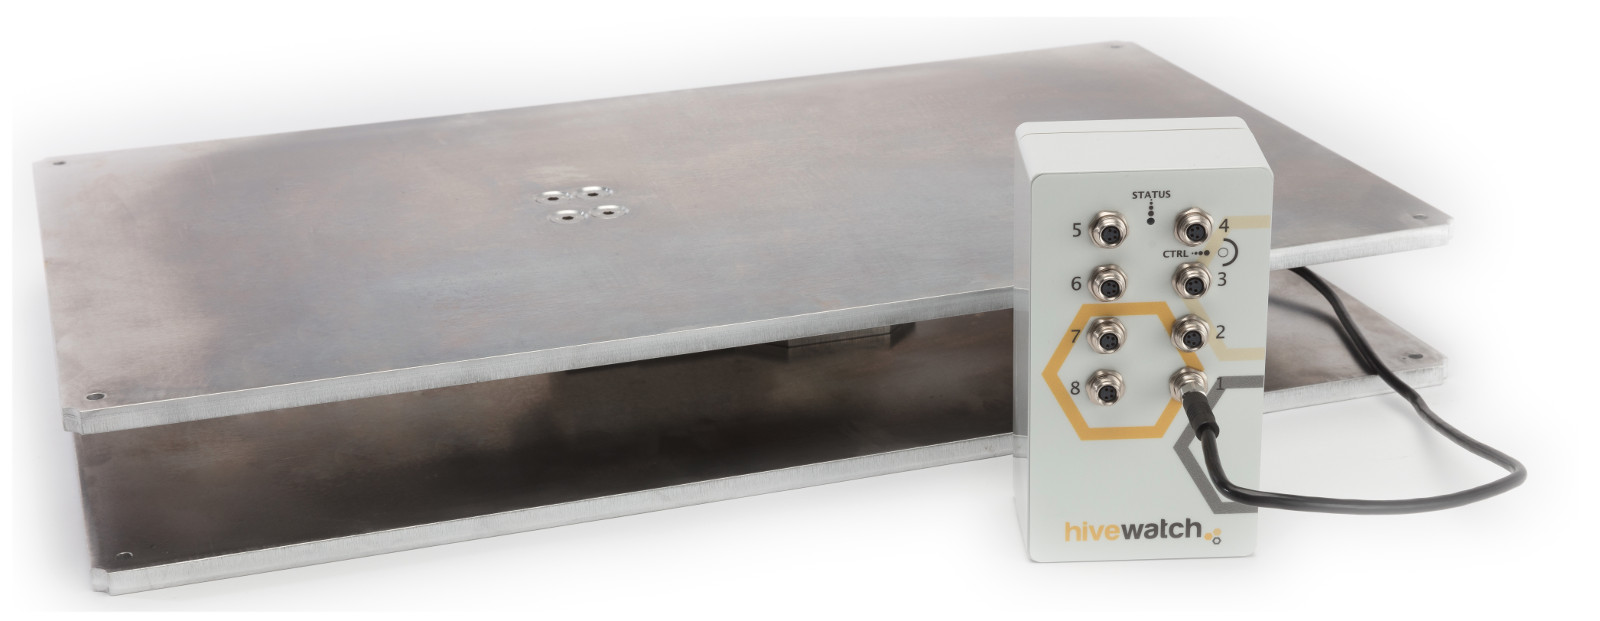
\includegraphics[width=0.75\textwidth]{figures/hivewatch_scale.jpg}
    \caption{HiveWatch System}
    \label{fig:hivewatch_scale}
\end{figure}

\textbf{Price:}
\begin{table}[ht]
    \centering
    \begin{bfhTabular}{lll}
       Expense & Price
       \\\hline
       Transmitter & CHF \num{385.00}\\\hline
       Scale & CHF \num{204.00} & \\\hline
       Brood Humidity Sensor & CHF \num{65.00}\\\hline
       Extension Cable & CHF \num{19.00} & \\\hline
       Subscription for 1 year & CHF \num{89.00}\\\hline
       \textbf{Total} &  \textbf{CHF 862.00}
    \end{bfhTabular}
    \caption{Price HiveWatch system}
    \label{tab:hivewatch_price}
 \end{table}

\newpage
\textbf{Interesting Features:}
\begin{itemize}
    \item HiveWatch is a modular system withing its own ecosystem. New scales can be added to the system with a proprietary connector. It seems like extending this system is plug-and-play.
    \item HiveWatch provides an app that can be used to monitor the weight of the beehive. The app also provides a history of the measured data.
    \item The beekeeper can set up alerts that will notify them if certain events occur. This includes, for example, if the scale thinks it detects a bee swarm.
\end{itemize}
\textbf{Problems:}
\begin{itemize}
    \item HiveWatch is a closed system. Interfaces are not documented, and the data is not accessible to the beekeeper by default. There is a forum where you can ask questions about the system. The developer seems to be reasonably active and provides information about the system, but this is not a good solution.
    \item It seems that the data is only accessible through the app. This makes it hard to analyze the data in a way that isn't intended by the developer.
    \item The solution is very expensive. The system also only seems to work if you have a subscription which is also very expensive.
\end{itemize}
\newpage

\subsubsection{Wolf-Waagen}

\begin{figure}
    \centering
    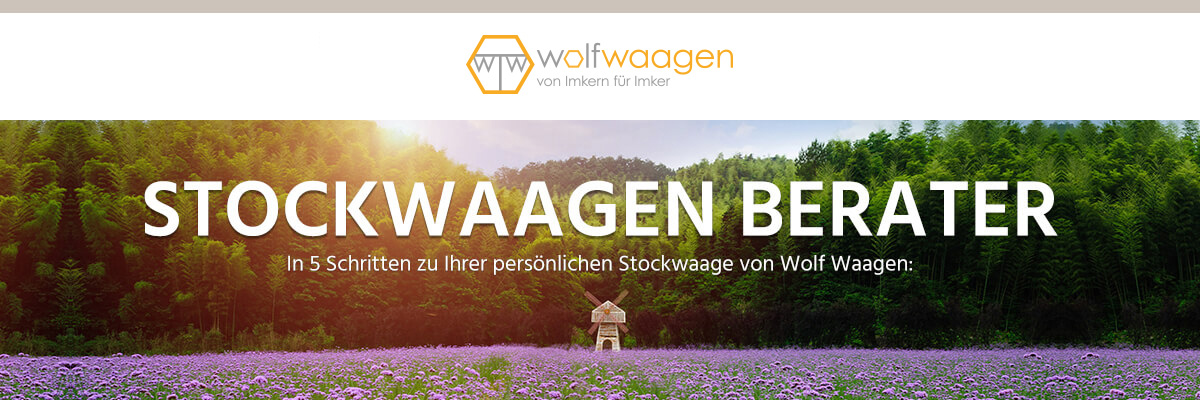
\includegraphics[width=1\textwidth]{figures/wolf_waagen_logo.jpg}
    \caption{Wolf-Waagen}
    \label{fig:wolf_waagen}
\end{figure}
Wolf-Waagen (Wolf-Scales) is a German business that specializes in bee scales. They sell a variety of scales that can be used to measure the weight of a beehive. They also have a diverse variety of sensors that can be used to collect additional data points like rainfall or wind. Furthermore, they provide a web interface that can be used to monitor the scales and provide an SMS altering service.

\begin{figure}
    \centering
    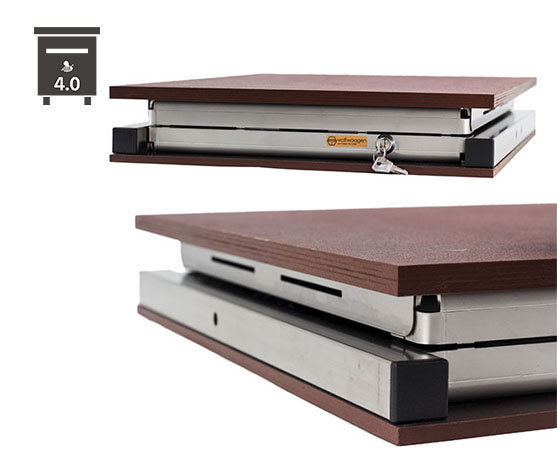
\includegraphics[width=0.75\textwidth]{figures/wolf_waagen_4.0.jpg}
    \caption{Wolf-Waagen System}
    \label{fig:wolf_waagen_4.0}
\end{figure}

\textbf{Price:}
Sadly, Wolf-Waagen doesn't give any exact information about pricing. They only specify the minimum price of the "ApiGraph4.0" scale, which is €\num{899.00}.
\begin{table}[ht]
    \centering
    \begin{bfhTabular}{lll}
       Expense & Price
       \\\hline
       ApiGraph4.0 & € \num{899.00}+\\\hline
       Software Service for 1 year & € \num{24.00} & \\\hline
       Data Plan for 1 year & € \num{15.00}\\\hline
       \textbf{Total} &  \textbf{CHF 938.00+}
    \end{bfhTabular}
    \caption{Price Wolf-Waagen system}
    \label{tab:tab1}
 \end{table}

\newpage
\textbf{Interesting Features:}
\begin{itemize}
    \item The scale appears to be really well-built. Most of the parts are made of metal and the scale looks really sturdy. Overall it seems like a good quality product. 
    \item Wolf-Waagen provides the option to connect additional sensors to the scale. It also seems like you can easily hook up additional scales to the system.
    \item They give you the option to have a diverse assortment of power sources. This includes solar panels, batteries, and a power adapter.
\end{itemize}
\textbf{Problems:}
\begin{itemize}
    \item Although the system seems to be really well-built, it is very expensive. The price of the scale is already very high, and the subscription and data plan are also very expensive.
    \item It looks like you have to completely rely on the Wolf-Waagen service. The data is not accessible to the beekeeper by default. The beekeeper can only access the data through the web interface. This makes it hard to analyze the data in a way that isn't intended by the developer.
\end{itemize}

\newpage

\subsection{Open Source Solutions}

There are a lot of open source projects that aim to solve the same problem. However, as with many open source projects, they are not very well documented and are not very easy to use. Also since they are often created by hobbyists, they are not general purpose solutions. They are often very specific to the needs of the creator. This makes it hard to use them in a real-world scenario.

Because of this, I decided to not use any of these solutions as is but to improve on existing concepts. I think that it is better to create my own solution easy to use and is suited to my needs.

\newpage

\subsection{Hardware Planning}
\subsubsection{Rough Setup}
In essence, the scale needs to provide a surface on which the beehive can be mounted and that measures the weight applied to it. This should be as low to profile as possible as not to interfere with any existing mounting equipment like standoffs or compartments in a bee house.

For this reason, I've decided to work with a simple, two plates approach. The first plate is the actual scale on which the beehive is mounted. The second plate is a baseplate to provide a stable foundation to the second plate. The load cells are mounted in between the two plates together with the load cell amplifier, so there is no need for any additional wiring and the scale can be connected to the microcontroller over a single cable.

The microcontroller is located in a separate housing, so it can be easily accessed without disassembling the scale. Any additional sensors or actuators can be connected to the microcontroller. In this case, I've decided to use a waterproof temperature sensor to be used inside the beehive as a proof of concept.

\subsubsection{Scale}
The baseplates are made out of wood and are 40 cm x 70 cm x 2 cm to accommodate a Swiss beehive. The have 4 holes in the corners to connect the plates to each other with the help of nuts, washers and bolts. The holes are countersunk to make sure that the nuts and bolt-heads are not protruding from the surface.

The four load cells are then glued to the baseplate with epoxy about 10 cm away from each edge and wired together.

\begin{figure}
    \centering
    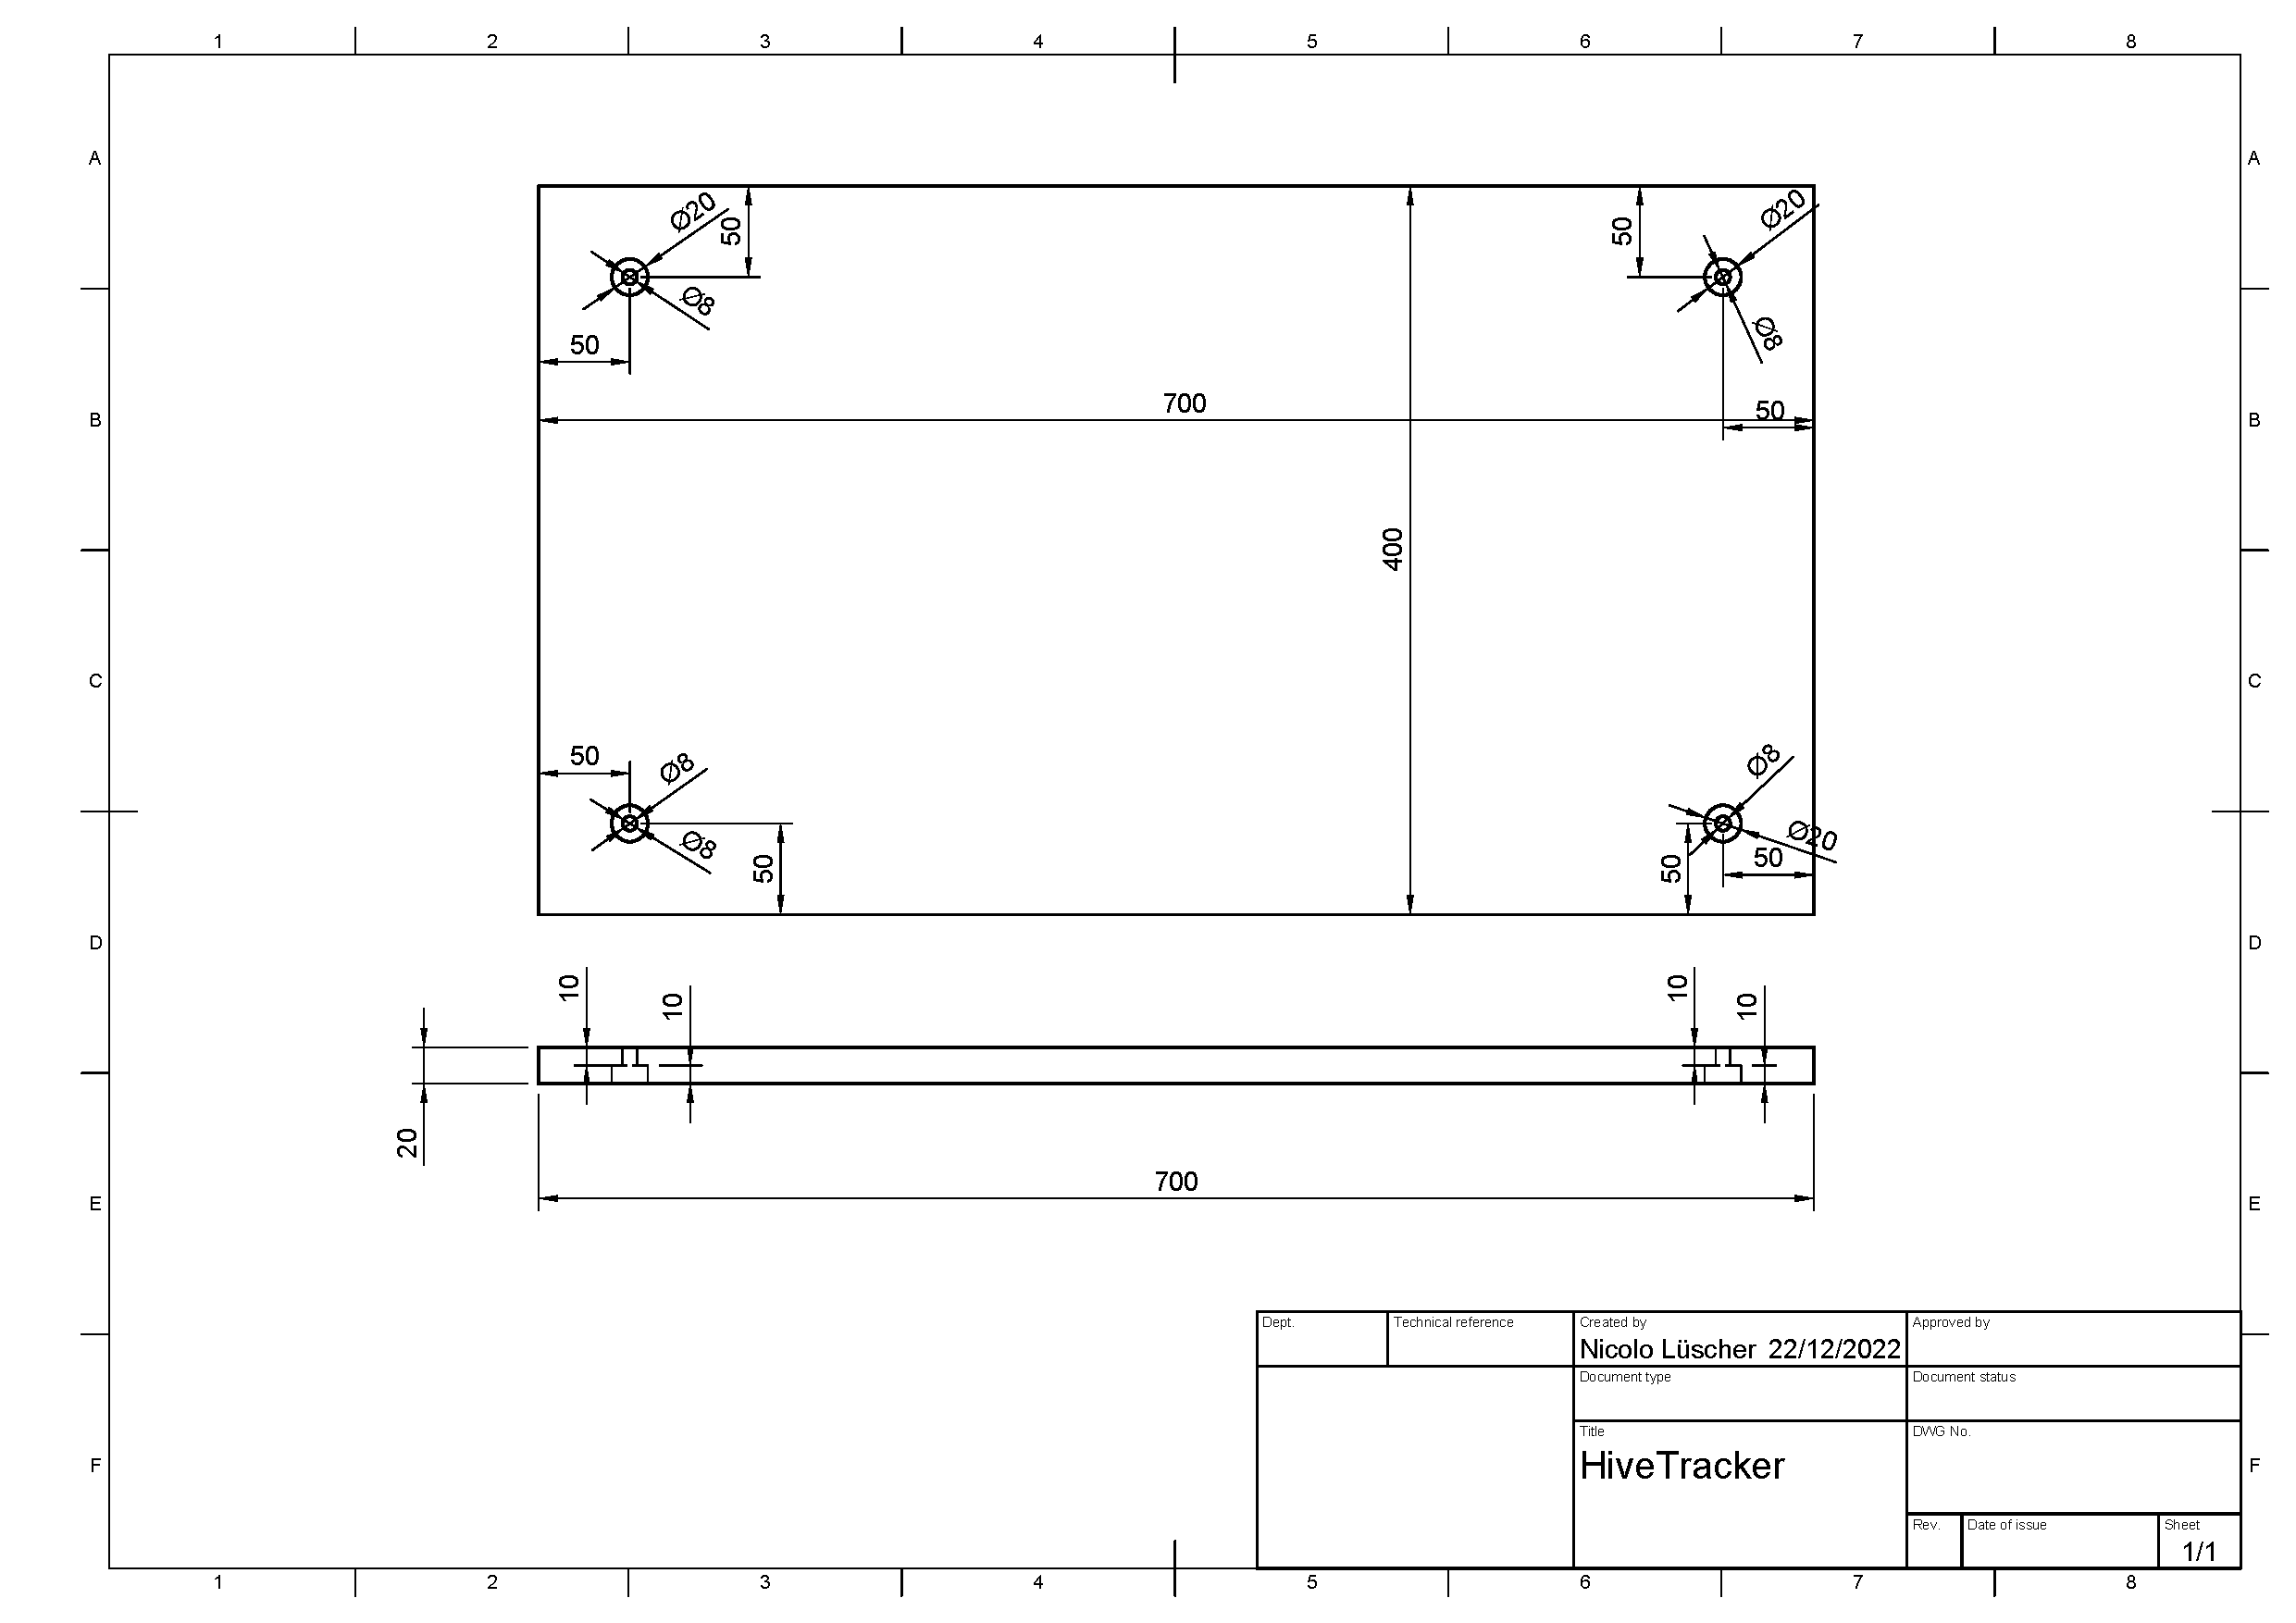
\includegraphics[angle=90,width=1\textwidth]{figures/hivetracker_baseplate.pdf}
    \caption{Baseplate Technical Drawing}
    \label{fig:baseplate_drawing}
\end{figure}
\newpage

\subsubsection{Load Cells}
The load cells used are a generic Chinese product normally used for human scales and are rated for 50 kg each. Since there are four of them, the maximum weight that can be measured is 200 kg. This is more than enough for a beehive.

\begin{figure}
    \centering
    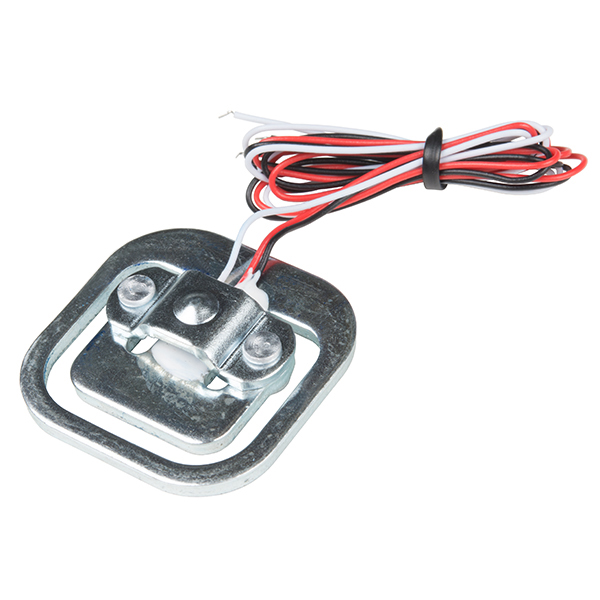
\includegraphics[width=0.5\textwidth]{figures/loadcell.jpg}
    \caption{Load Cell}
    \label{fig:loadcell}
\end{figure}

\newpage
\subsubsection{Load Cell Amplifier}
The load cells are connected to a HX711 load cell amplifier. It is used to read the measurements from the load cells and convert them into usable data. The amplifier is connected to the microcontroller.

\begin{figure}
    \centering
    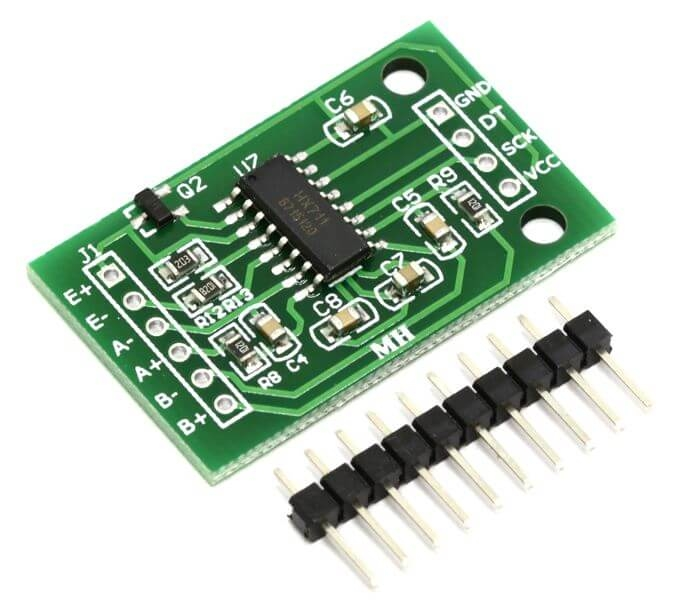
\includegraphics[width=0.5\textwidth]{figures/hx711.jpg}
    \caption{Load Cell Amplifier}
    \label{fig:loadcell_amplifier}
\end{figure}

\newpage
\subsubsection{Temperature Sensor}
The temperature sensor is a DS18B20 waterproof temperature sensor with a 3 m cable. It is connected to the microcontroller and can be used to measure the temperature inside the beehive.

\begin{figure}
    \centering
    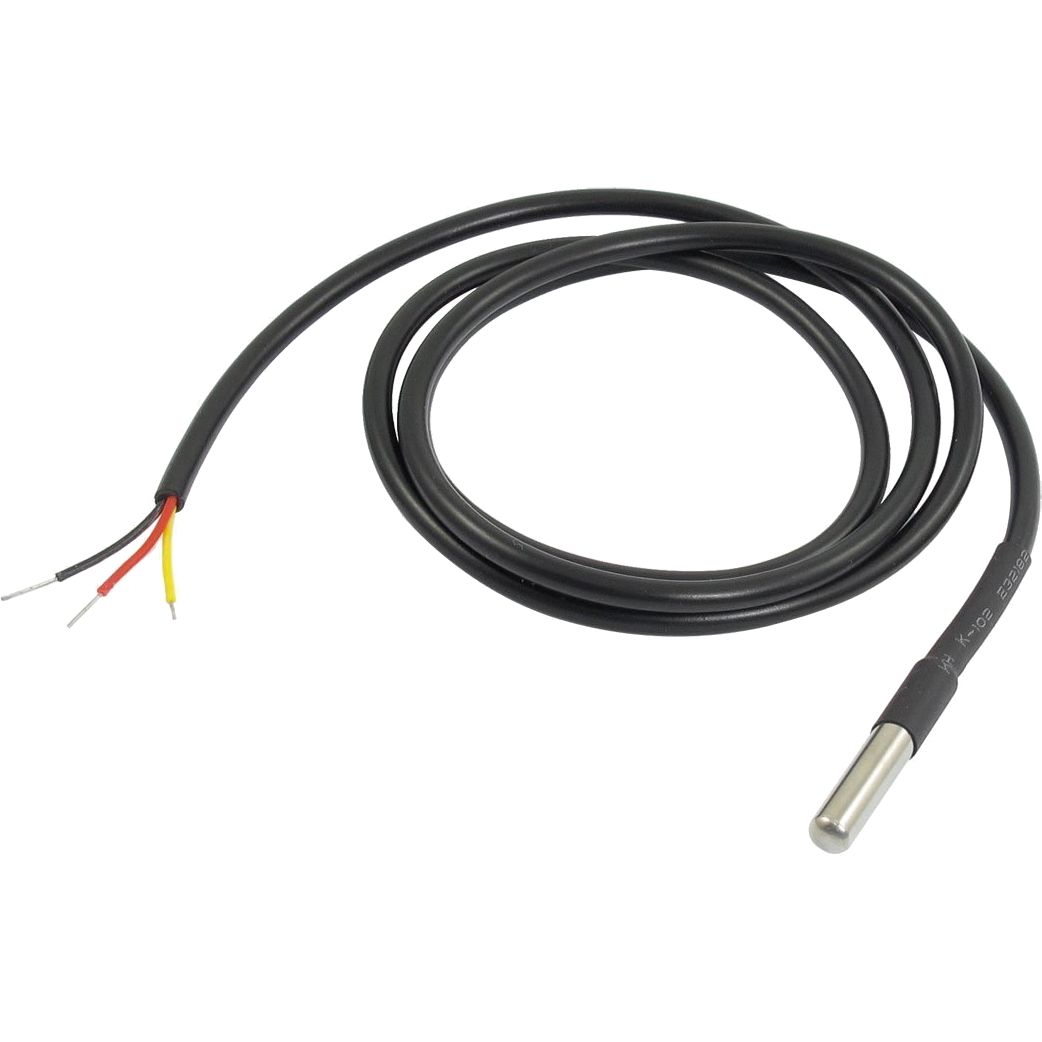
\includegraphics[width=0.5\textwidth]{figures/DS18B20.png}
    \caption{Temperature Sensor}
    \label{fig:temperature_sensor}
\end{figure}
\newpage
\subsubsection{Microcontroller}
The microcontroller is LILYGO® TTGO T-Call V1.4 ESP32 Wireless Module with a built-in SIM800L Module for GSM/GPRS. It is already capable to connect the internet via a SIM card out of the box, and it can be powered by a 3.3V - 5V DC power source, making it possible to use a wide variety of power sources. The documentation is quite poor, mostly consisting of a Chinese data sheet and a few examples. However, it is possible to use the Arduino IDE to program it, which makes it easy to use since all the necessary libraries to use the load cell amplifier and the temperature sensor are already included.

\begin{figure}
    \centering
    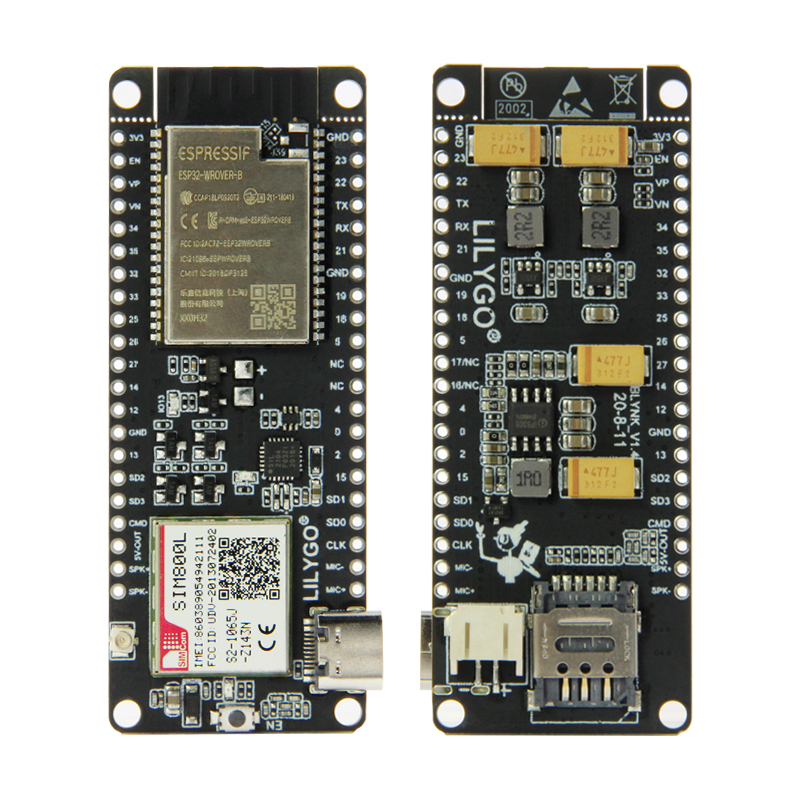
\includegraphics[width=0.5\textwidth]{figures/esp32.jpg}
    \caption{LILYGO® TTGO T-Call V1.4 ESP32 Wireless Module Microcontroller}
    \label{fig:esp32}
\end{figure}

\newpage
\subsection{Software Planning}

\subsubsection{Architecture}
The software is split into five different components. These components should be connected to each other via a simple interface, so that it is easy to replace any of them with a different implementation.
The components are:
\begin{itemize}
    \item Sensor Block
    \item Data Broker
    \item Backend
    \item Database
    \item User Interface
\end{itemize}

\begin{figure}
    \centering
    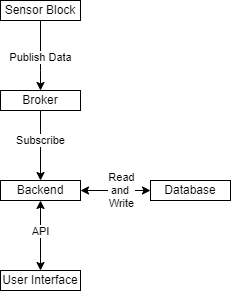
\includegraphics[width=0.5\textwidth]{figures/hivetracker_software_architecture.png}
    \caption{Software Architecture}
    \label{fig:software_architecture}
\end{figure}

\subsubsection{Sensor Block / ESP32 Firmware}
The sensor block runs the ESP32 firmware. The ESP32 firmware is written in C++ and uses the Arduino framework. It implements several libraries to interact with the hardware. Refer to section \ref{sec:firmware} for more information.

\subsubsection{Data Broker}
Data between the sensor block and the backend is exchanged via a data broker. The data broker is a simple MQTT broker. The sensor block publishes the data to the broker and the backend subscribes to this data. The data broker is implemented using the Mosquitto MQTT broker. Refer to section \ref{sec:data_broker} for more information.

\subsubsection{Backend}
The backend listens for data coming from the sensor block by subscribing to the data broker. If there is new data, it is timestamped and stored in the database. The backend also provides an API that can be used by the frontend to receive data from the database and make changes to the calibration information used to calibrate the scale. The backend is implemented using Node.js and Express. Refer to section \ref{sec:backend} for more information.

\subsubsection{Database}
The database is used to store all data related to the beehive. It makes the otherwise ephemeral data persistent and allows to query it. The database is implemented using Postgres. Refer to section \ref{sec:database} for more information.

\newpage
\section{Implementation}


\subsection{Prototype}
\subsubsection {Hardware} \label{sec:hardware}
The first step was to build the hardware of the prototype. For this I first had to build the scale itself.

For this I cut out the baseplates from wood according to my technical drawing and then drilled the required holes for the nuts and bolts. I then glued the load cells to the baseplates and wired them together as seen in figure \ref{fig:loadcell_wiring}. I had to drill some shallow relief holes I did not account for in my design because the load cells had a small protrusion and wouldn't have laid flush otherwise. Furthermore, I then connected the load cells to the load cell amplifier and the load cell amplifier to the microcontroller.

\begin{figure}
    \centering
    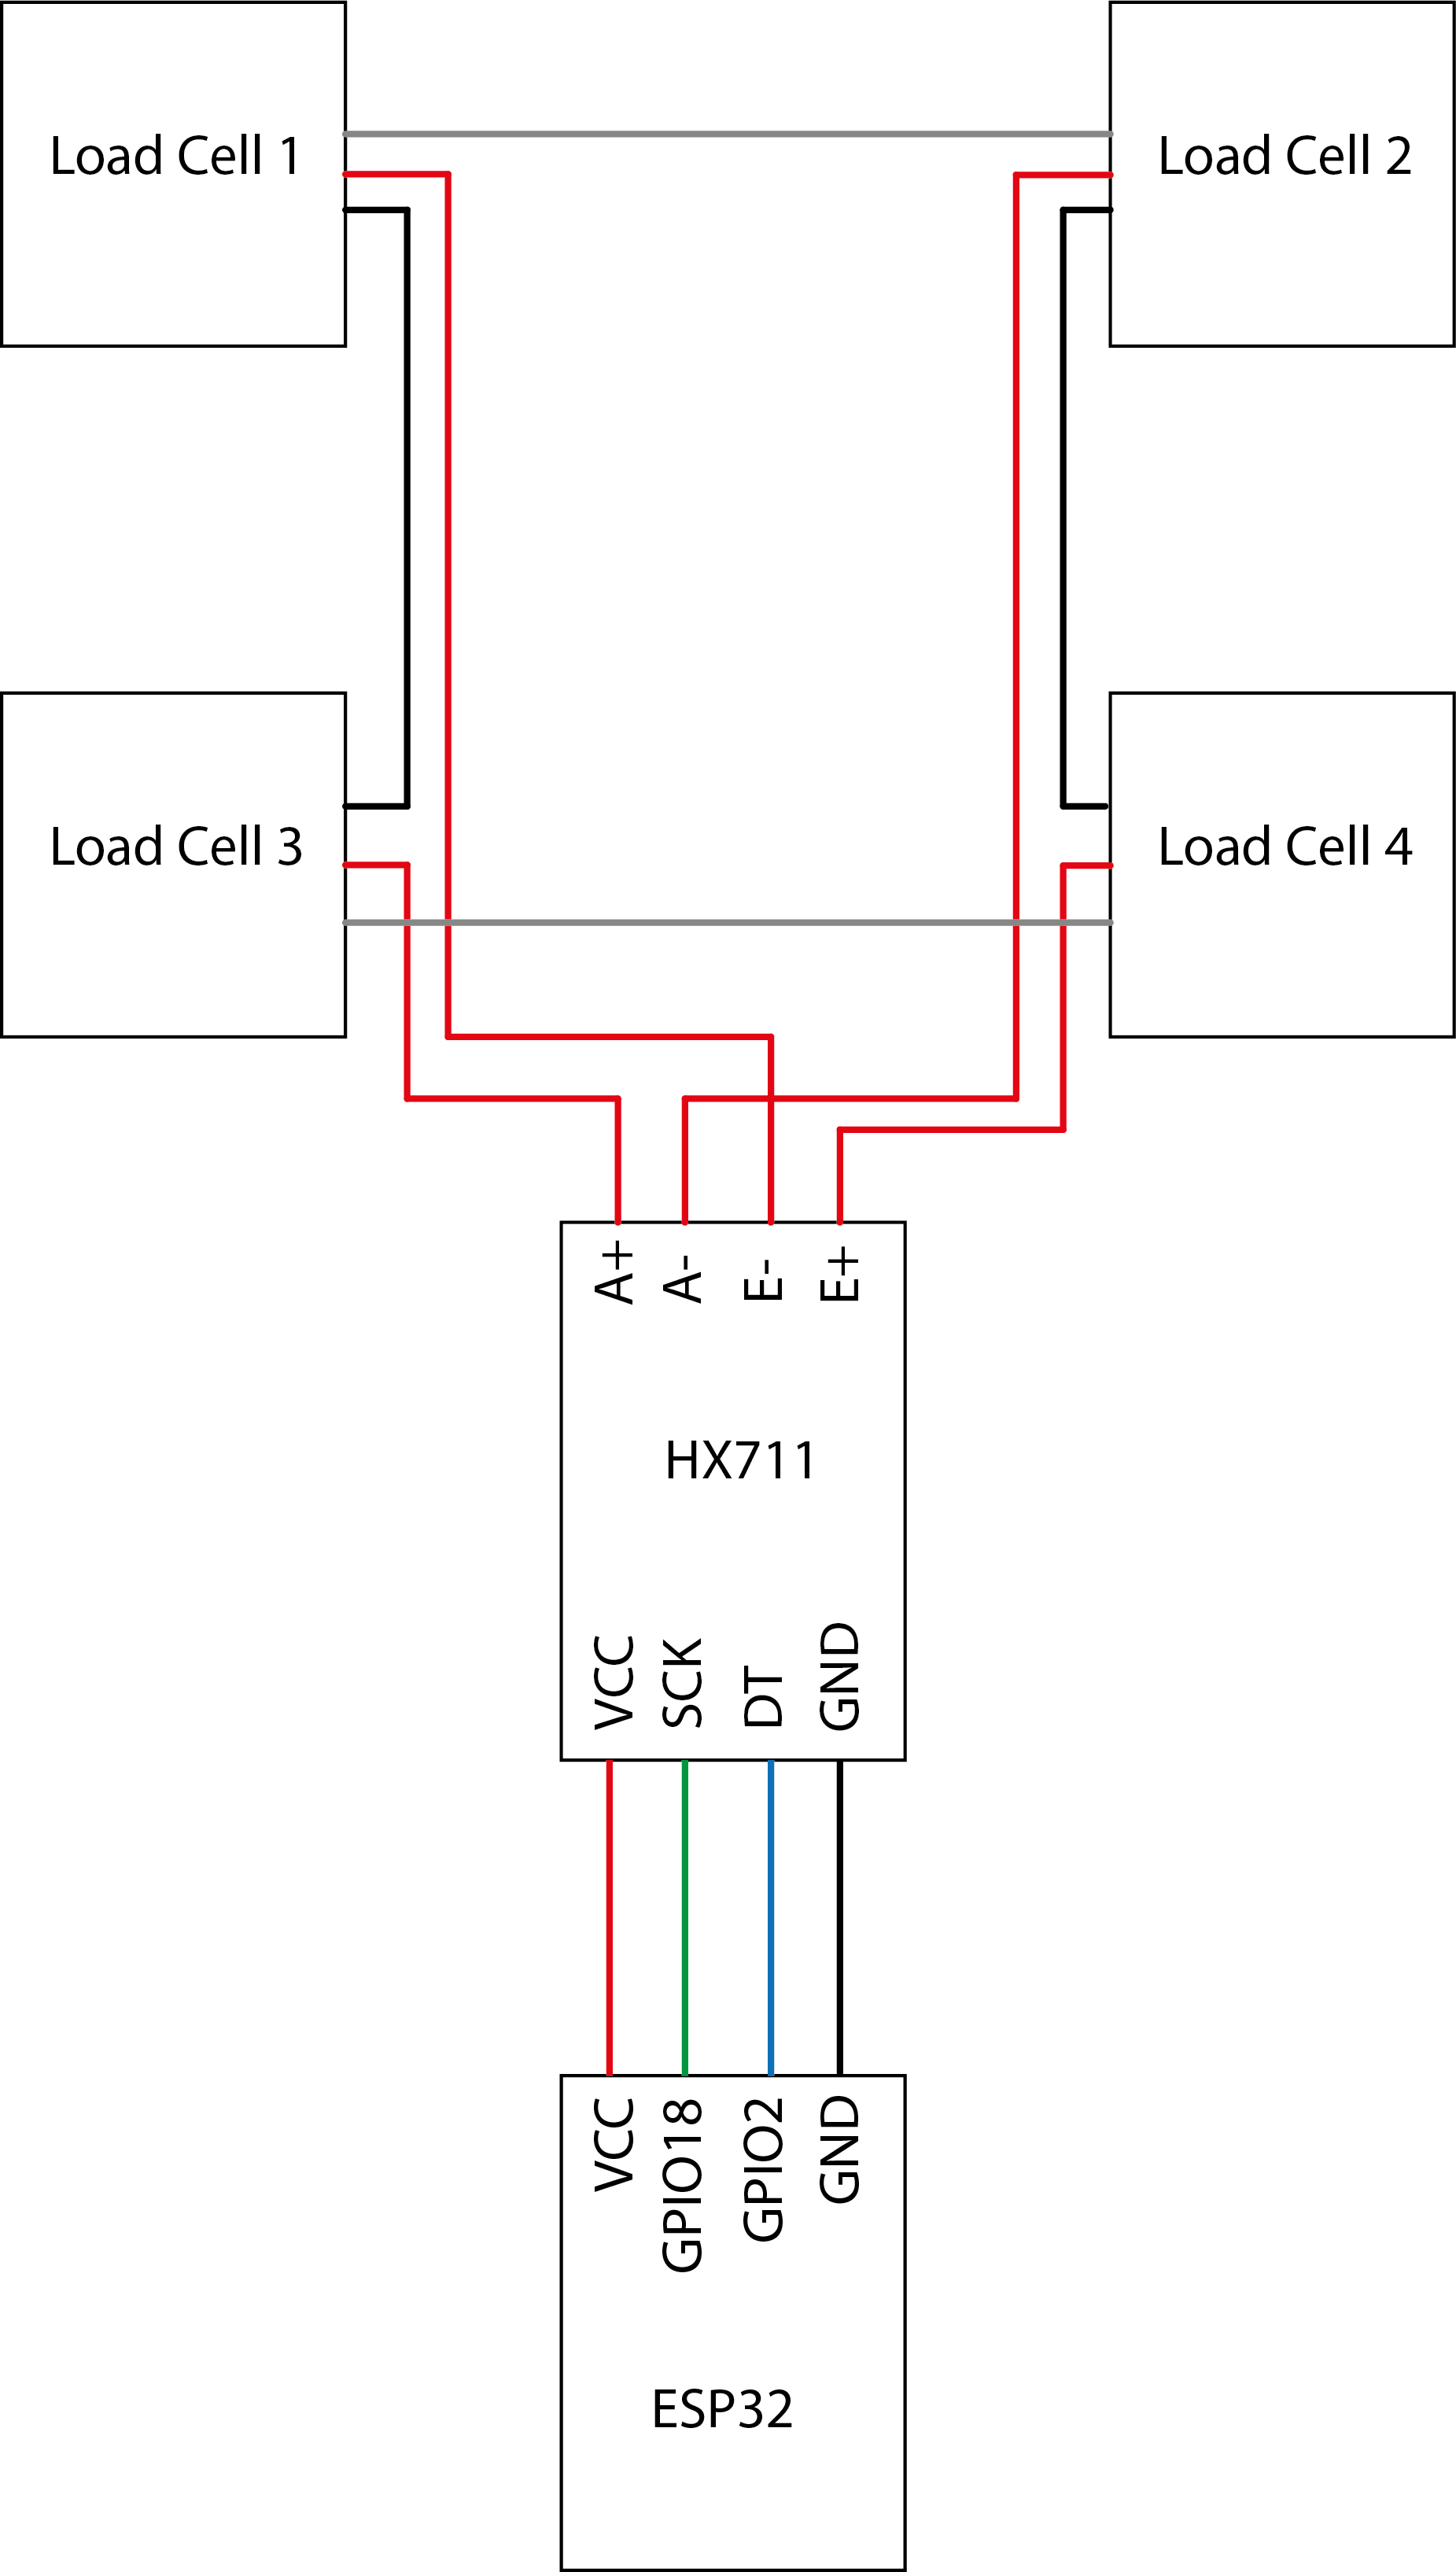
\includegraphics[width=0.5\textwidth]{figures/loadcell_wiring.png}
    \caption{Baseplate Prototype}
    \label{fig:loadcell_wiring}
\end{figure}

After that, I glued some squares cut from hard plastic and glued them to the baseplate without the load cells at the contact points of the load cells. This is to prevent the load cells from digging into the wood and to make sure that the load cells are not damaged by the wood. I then placed the two plates on top of each other and bolted them together.

I then tested the scale for accuracy and repeatability. I found that the scale was not suited for quick measurements, since it takes a few seconds for the load cells to settle. My guess is that this is due to stress in the wood. However, it is accurate enough for my purposes since I am interested in the change in weight over time, not the absolute weight at a given moment.

After this I connected the temperature sensor to the microcontroller. For this, I had to solder a 4.7 k\Omega resistor to the temperature sensor and connect it to the microcontroller as seen in figure \ref{fig:temperature_wiring}. I then tested the temperature sensor and found that it was very accurate.

\begin{figure}
    \centering
    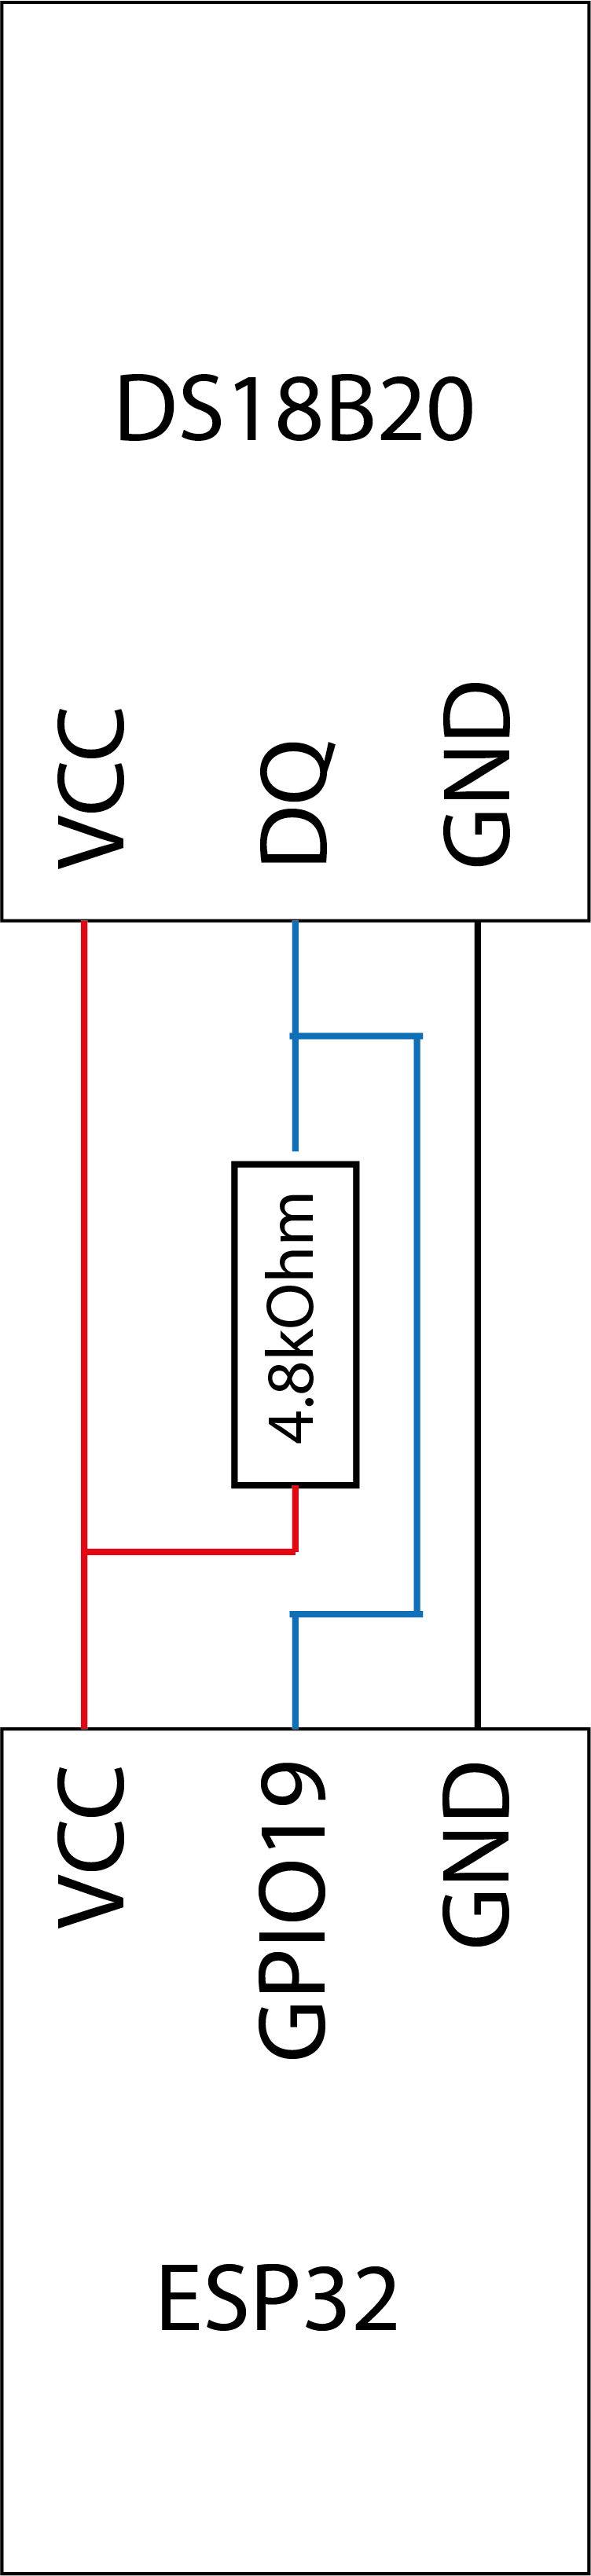
\includegraphics[angle=270,width=1\textwidth]{figures/temperature_wiring.png}
    \caption{Temperature Sensor Prototype}
    \label{fig:temperature_wiring}
\end{figure}

\newpage
\subsubsection {Firmware} \label{sec:firmware}
The firmware is written in C++ and uses the Arduino framework and is used to get the data from the sensors to the data broker.

Simplified, the firmware performs the following steps:

\begin{enumerate}
    \item Determine the board type and set up the hardware accordingly
    \item Set configuration values
    \item Establish a connection to the GSM network via the SIM800L module
    \item Set up a connection to the data broker via MQTT
    \item Initialize the temperature Sensor
    \item Initialize the load cell amplifier
    \item Read the Temperature
    \item Read the Weight
    \item Write the data to the data broker
    \item Disconnect from the data broker
    \item Disconnect from the GSM network
    \item Enter deep sleep mode for a given amount of time
    \item Wake up and repeat
\end{enumerate}

Refer to appendix \ref{lst:firmware} for the full source code of the firmware.

\subsection{Server Setup}
\subsubsection {Data Broker} \label{sec:data_broker}
For easy deployment, I decided to use a docker container for the data broker. I used the official Mosquitto docker image and configured it to use a password file for authentication. I also configured it to use TLS encryption. Refer to appendix \ref{lst:mosquitto-conf} for the configuration file and to appendix \ref{lst:mqtt-docker-compose} for the docker compose file.

This broker provides standard MQTT functionality and is used to exchange data between the sensor block and the backend. The sensor block publishes the data to a topic on the broker and the backend subscribes to this topic. This means that the backend automatically gets notified when new data is available and doesn't have to poll the broker for new data.

\subsubsection {Backend} \label{sec:backend}
The backend persists the data coming from the data broker and makes it available to the user interface. It is implemented using Node.js and Express. It uses the MQTT.js library to connect to the data broker and uses Sequelize to interact with the database. Refer to appendix \ref{sec:backend} for the relevant source code of the backend.

\textbf{Node.js} is a JavaScript runtime that allows to run JavaScript code outside the browser. This makes it possible to implement server side code in JavaScript. It also provides a package manager that allows to easily install and manage dependencies called NPM (Node Packet Manager). In this project, Node is used to handle incoming HTTP requests and to interact with the database. 
It exposes an API that allows to query the database and to retrieve the data to be displayed in the user interface. There are also endpoints that allow to update the configuration of the beehive. This includes a server side method to calibrate the scale and set a zero offset. Refer to appendix \ref{lst:app.js} for the relevant source code of the backend.

\textbf{Express.js} is a web framework for Node.js that allows to easily implement HTTP endpoints. It provides a simple API to define the endpoints and to handle incoming requests. It also provides a middleware system that allows to easily add functionality to the endpoints. Express.js provides an easy way to implement backend routing and greatly simplifies the code structure and the endpoint management.

\textbf{Sequelize} is an ORM (Object Relational Mapper) that allows to interact with the database using JavaScript objects. It provides a simple API to define the database schema and to interact with the database. It also provides a migration system that allows to easily update the database schema. This is useful for example when new data is added to the database or when the data format changes. It also allows to easily query the database and to retrieve the data in a format that is easy to use in the user interface without having to write any SQL queries. Refer to appendix \ref{lst:database.js} for the database schema.
Sequelize adds the "createdAt" and "updatedAt" field to any data entry by default and automatically updates them when the data is changed. This further simplifies the backend code.

\textbf{MQTT.js} is a library that allows to connect to an MQTT broker and to subscribe to topics. It also provides an API to publish data to a topic. It is used to connect to the data broker and to subscribe to the topic that the sensor block publishes to. The backend is then automatically notified when new data is available and can act accordingly.

\textbf{Networking}
The backend and the frontend are intended to be deployed on the same machine. To simplify the port management, a reverse proxy is used to route all API requests to the backend and all other requests to the frontend. This is done using the Angular reverse proxy. This allows the machine to only expose port 80 and 443 to the internet and handle the rest internally making it easier to implement TLS encryption.

\subsubsection {Database} \label{sec:database}
The database is used to store data related to the project. It is implemented using PostgreSQL and is managed using Sequelize. It is running in a docker container and is exposed to the backend via a docker network making it easy to deploy and manage. The same docker container is also running an Adminer instance that allows to easily manage the database. Refer to appendix \ref{lst:database-docker-compose.yml} for the docker compose file.

\newpage
\subsection{User Interface}\label{sec:user_interface}
The system is designed to make it user interface agnostic. This means that the user interface can take any shape and form as long as it can interact with the backend over the provided API endpoints. This allows to easily implement different user interfaces for different use cases. For example, a user interface for a mobile phone and a user interface for a desktop computer. This also allows to easily implement different user interfaces for different users. For example, a user interface for the beekeeper and a user interface for the bee researcher.

The user interface I've implemented for this project is a simple web application that allows to view the data coming from the beehive. The user is also able to update the configuration of the beehive. This includes a method to calibrate the scale and set a zero offset and therefore provides all the functionality to set up the beehive.

The user interface is implemented using \textbf{Angular} and is deployed using the Angular reverse proxy. This is a bit overkill for this project, but it allows to easily extend the user interface in the future by providing a simple way to add new pages, components and services. For styling, \textbf{TailwindCSS} is used. It provides a simple, low CSS way to style the user interface with a result focused, fast approach.

\begin{figure}
    \centering
    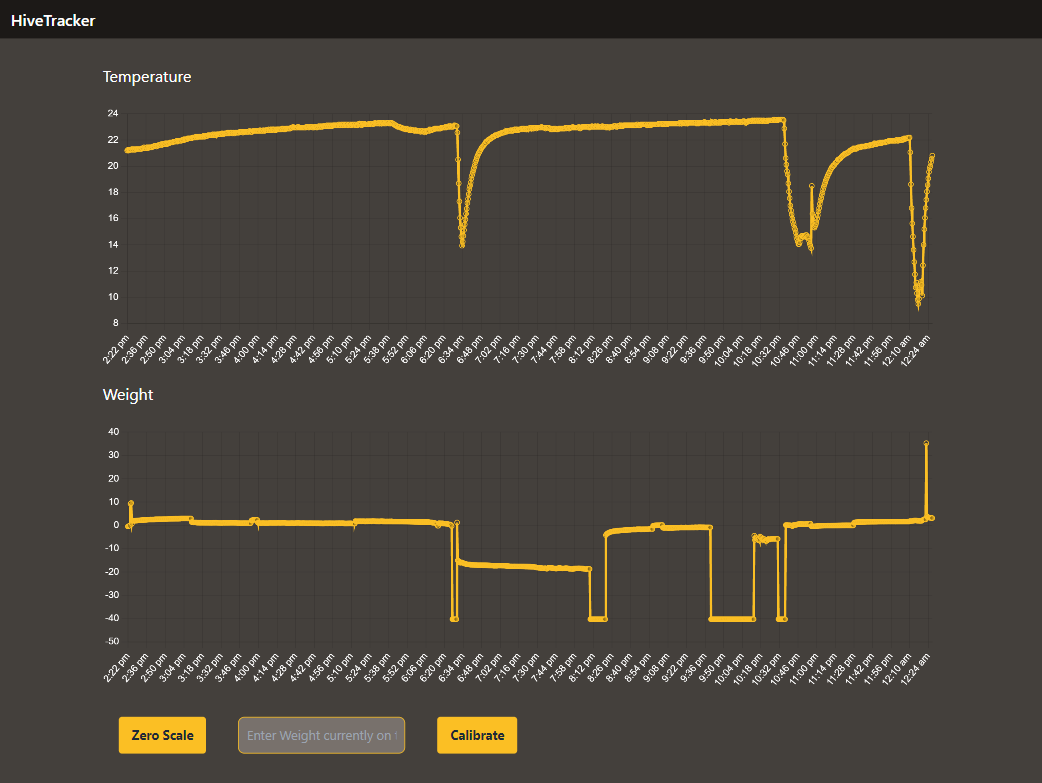
\includegraphics[width=0.8\textwidth]{figures/user_interface.png}
    \caption{Screenshot of the user interface}
    \label{fig:user_interface}
\end{figure}

\newpage
\section{Testing}
\subsection{Hardware Testing}
\subsection{Power Consumption}
\subsection{Software Testing}
\chapter{Results}
\section{System}
During the building process it became more and more clear that this project would be more of a proof of concept other than a fully fetched, commercially viable product. There are just too many factors and variables that need to be considered in building a long-lasting, reliable, off-the-grid, weatherproof, accurate measuring system. For this reason, the system was more of a proof of concept than a fully fledged product and still needs some improvements to be made before it can be used in a real-world scenario.

Nonetheless, the resulting system fulfilled most of the requirements outlined in the planning phase and provides a solid base to be improved upon in the future. It fulfills its core functionality goals of collecting measurements of a beehive in a remote location and transmitting them to a central server where it can be accessed by a user interface. 

\begin{figure}
    \centering
    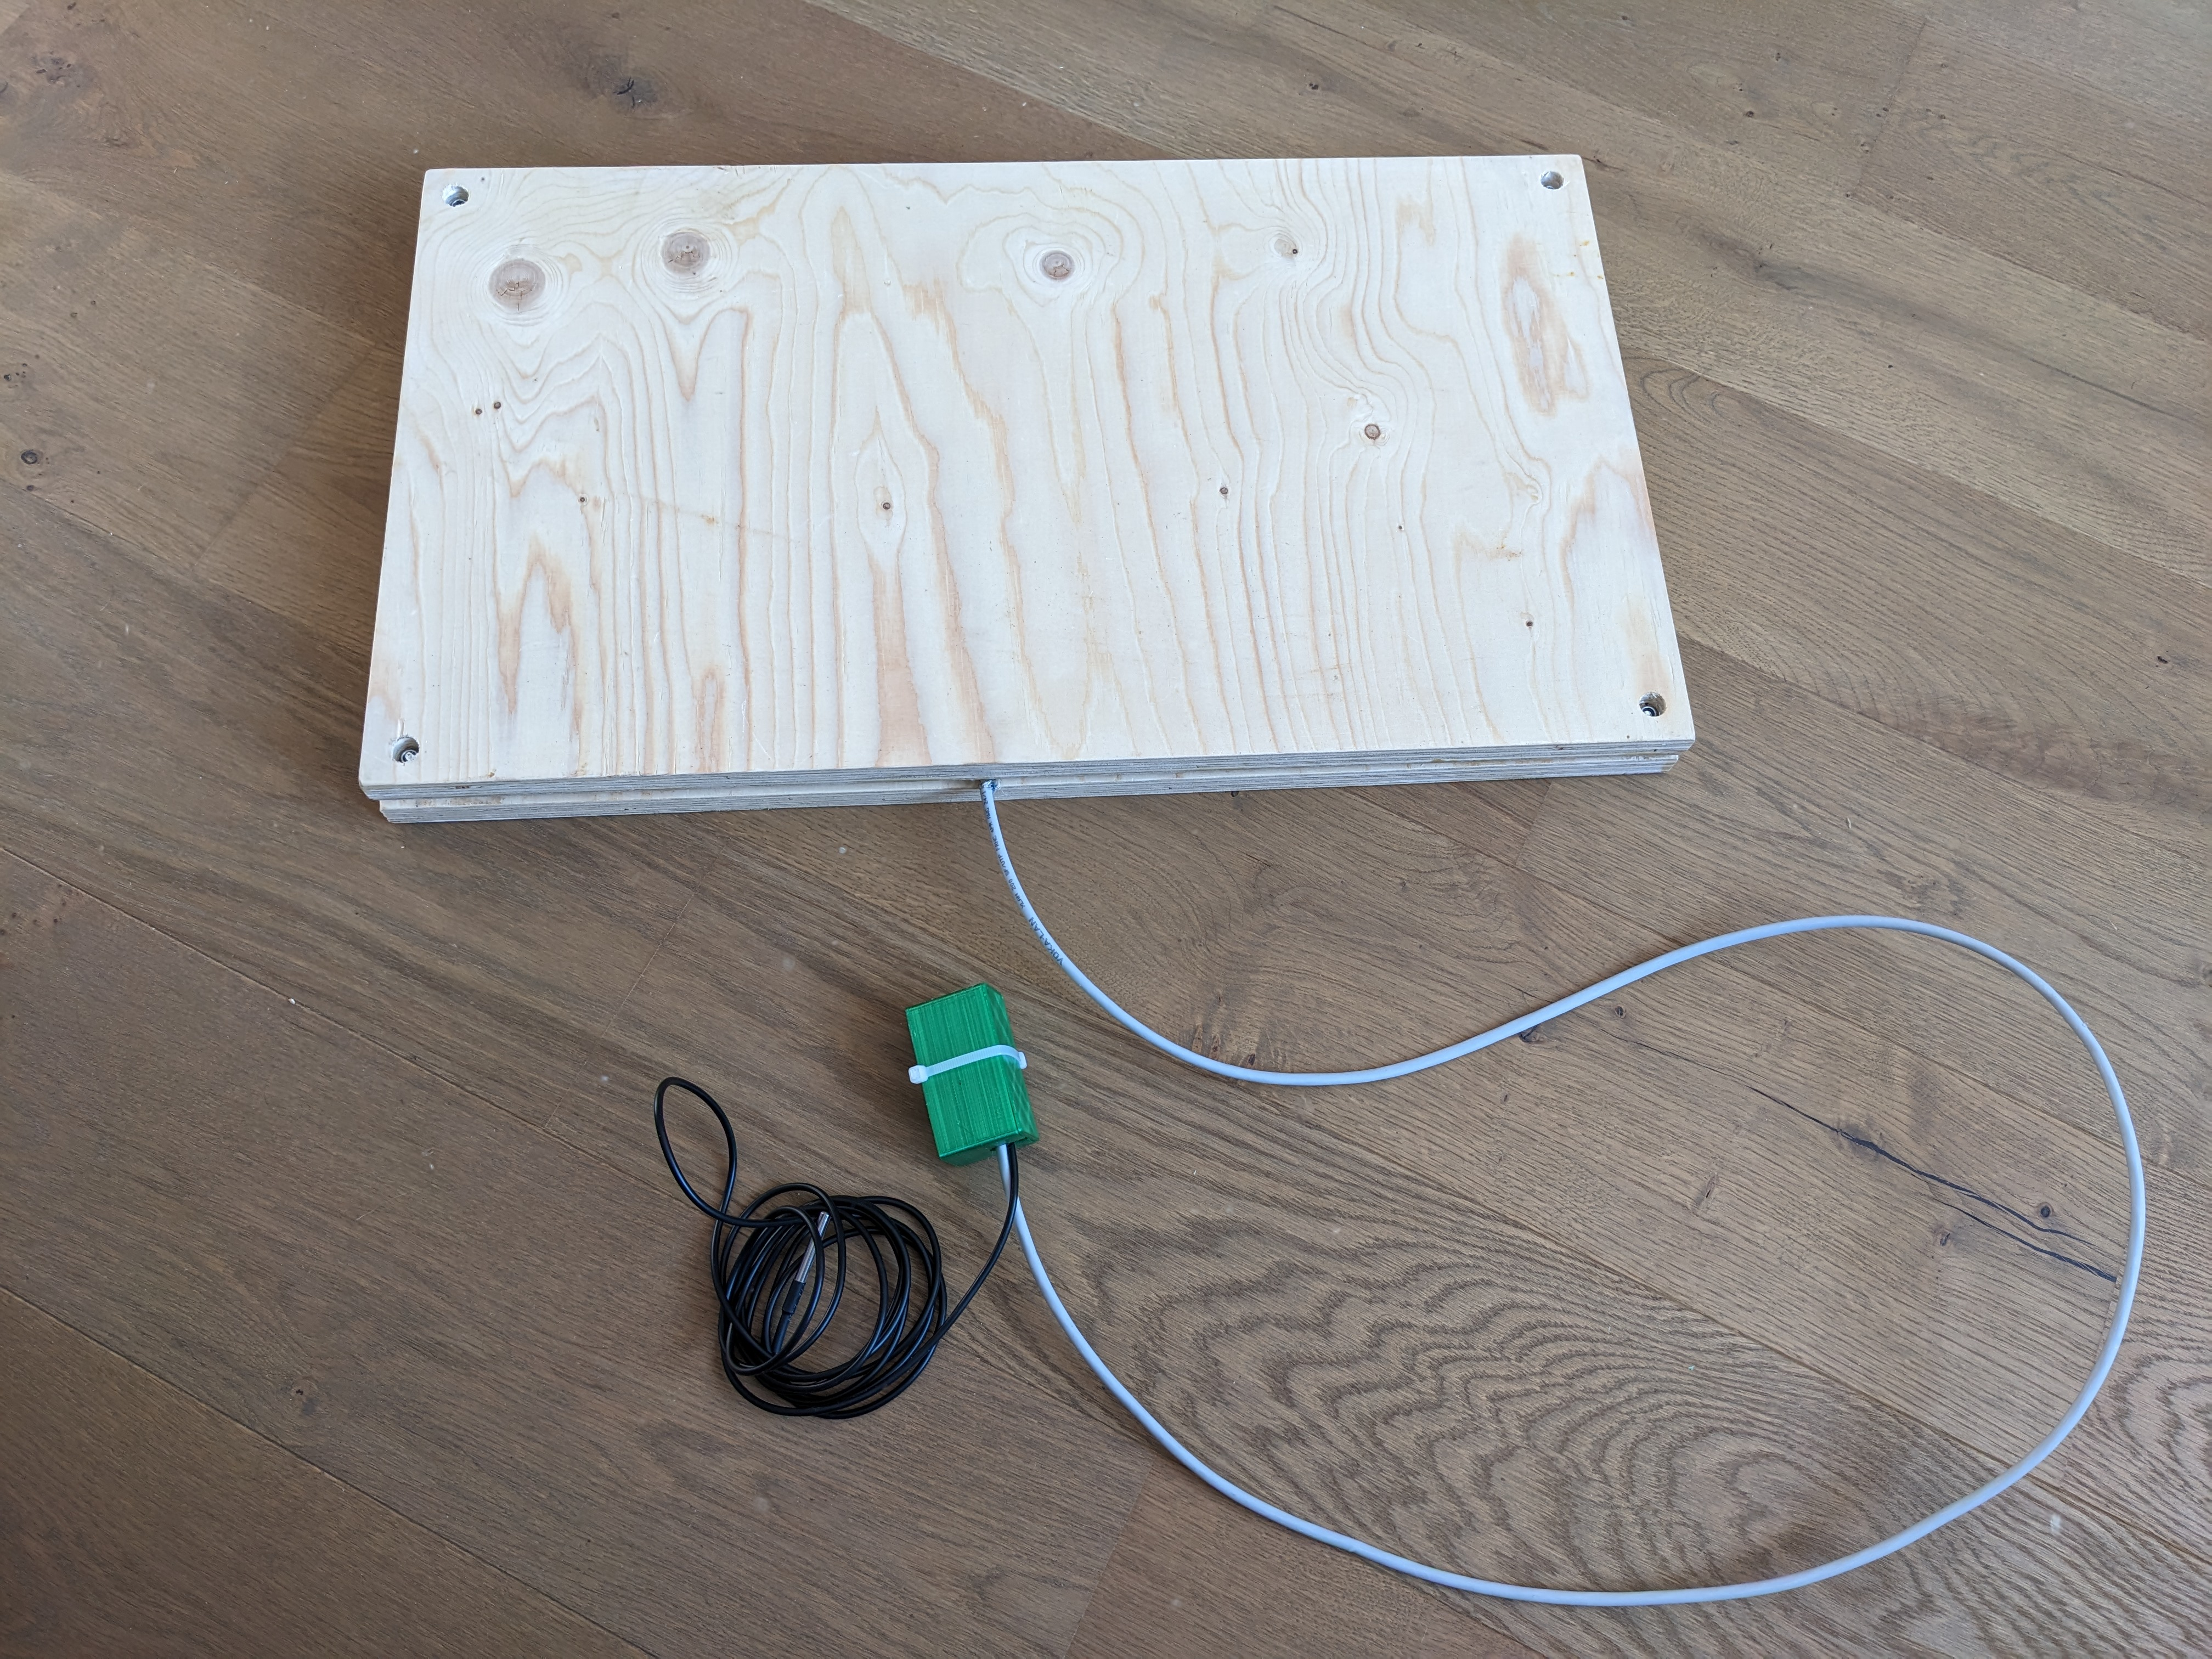
\includegraphics[width=0.55\textwidth]{figures/scale.jpg}
    \caption{Overview of the system}
    \label{fig:overview}
\end{figure}

\begin{figure}
    \centering
    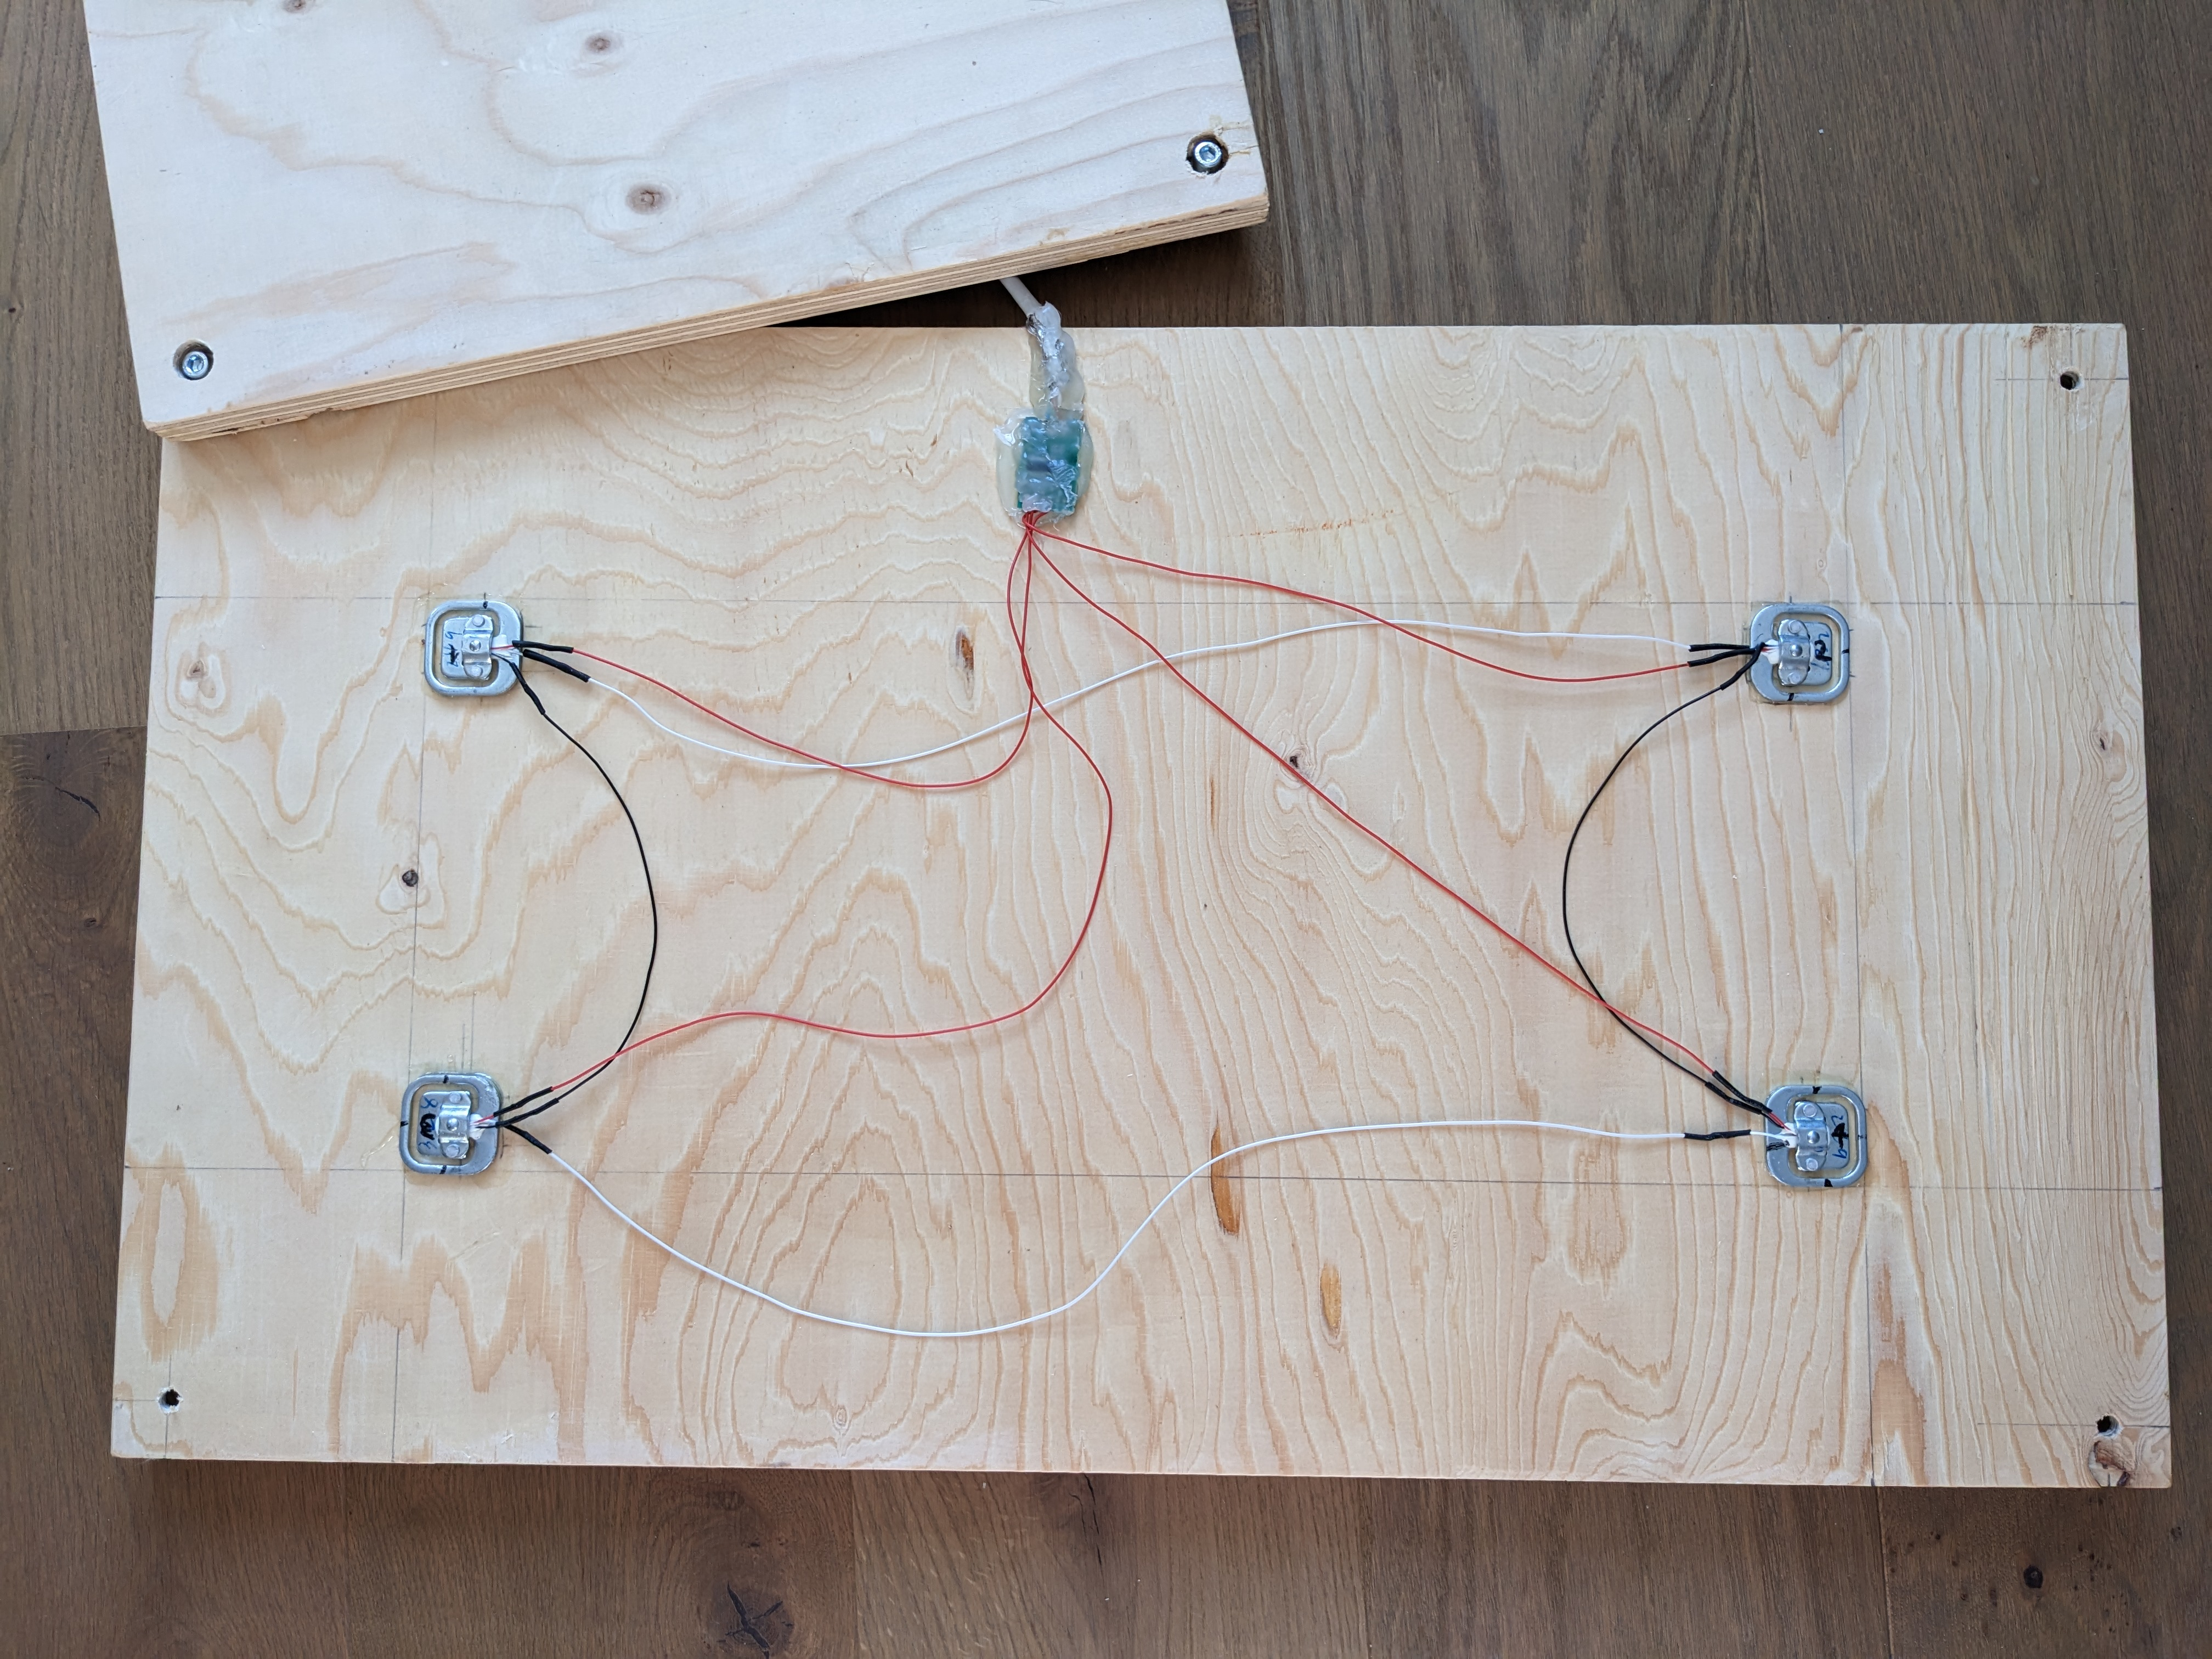
\includegraphics[width=0.55\textwidth]{figures/scale_wiring.jpg}
    \caption{Internal wiring of the scale}
    \label{fig:overview}
\end{figure}

\begin{figure}
    \centering
    \includegraphics[width=0.55\textwidth]{figures/esp32_connected.jpg}
    \caption{Internal wiring of the microcontroller}
    \label{fig:overview}
\end{figure}

\newpage
\newpage
\section{Costs}
The main goal of this project was to build the system as cost-effective as possible. The following table shows the total cost it took to build the system.

\begin{table}[ht]
    \centering
    \begin{bfhTabular}{llll}
       Name & Quantity & Price & Total
       \\\hline
       Wood & \num{1} & CHF\num{41.00} & CHF\num{41.00}\\\hline
       Wood Treatment & \num{1} & CHF\num{3.00} & CHF\num{3.00}\\\hline
       Cables & \num{1} & CHF\num{3.00} & CHF\num{3.00}\\\hline
       Temperature Sensor (DS18B20) & \num{1} & CHF\num{10.90} & CHF\num{10.90}\\\hline
       18650 LiPo Battery & \num{4} & CHF\num{8.90} & CHF\num{35.60}\\\hline
       LiPo Battery 4x Shield & \num{1} & CHF\num{16.90} & CHF\num{16.90}\\\hline
       Generic Load Cell & \num{4} & CHF\num{4.50} & CHF\num{18.00}\\\hline
       HX711 Load Cell Amplifier & \num{1} & CHF\num{4.50} & CHF\num{4.50}\\\hline
       LILYGO TTGO T-Call ESP32 SIM800L & \num{1} & CHF\num{25.17} & CHF\num{25.17}\\\hline
       Misc. Nuts, Bolts and other consumables & \num{1} & CHF\num{10.00} & CHF\num{10.00}\\\hline
       Data Plan for 365 Days & \num{1} & CHF\num{44.00} & CHF\num{44.00}\\\hline
        &  & \textbf{Total} & \textbf{CHF212.07}\\\hline
    \end{bfhTabular}
    \caption{Price of the system}
    \label{tab:tab1}
 \end{table}

This is way cheaper that even the cheaper commercially available beehive monitoring systems with the added benefit of being completely open source and customizable. This price doesn't include the time it took to build the system, which is a significant factor in the total cost of the system. Most of the time however was spent on the design, planning and research phase, which wouldn't need to be done again  for future iterations of the system.

 \newpage
\section{Conclusion}
\subsection{Future Improvements}
The system as it is right now is not really usable in the way it was intended. There are still some major improvements that need to be done like changing the material of the scale to something less subjectable to thermal expansion and addressing the load cell inaccuracies. Another important aspect is creating a weatherproof housing for the microcontroller and the batteries.

Another important aspect is providing solar power to the batteries. This would reduce the need for frequent battery changes and would make the system more reliable.

More user interfaces like SMS/Email notifications would also be a nice addition to the system.

Another interesting future prospect would be the addition of data analysis to the system. This would allow the user to get a better understanding of the data collected by the system and would allow for better decision-making. There could also be systems to make predictions about the future based on the data collected. For example a prediction of when the honey will be ready to harvest and how much the expected yield will be. Another system would be the prediction and detection of a swarm. This would allow the user to take action before the swarm leaves the hive and would allow for better swarm management.

\newpage
\subsection{Reflection}
All in all I think this project was a success. I was able to come up with a setup that did what it was supposed to do. Furthermore, I have learned a lot about designing and building IOT projects and the technologies used in the project. I am looking forward to improving the system in the future and transform it into a completely viable product. It is also my intention to make the system open source and share it with the community.

During the project, I've encountered some quite significant roadblocks, that I was able to overcome. I believe that this greatly improved my problem-solving skills and my ability to work under pressure. A lot of the problems I encountered were in fields I had no experiences in, which made it even more challenging. But I believe that solving those issues and thinking about the problems that arose made me a better engineer.

In conclusion, I really enjoyed working on this project, and I am looking forward to start working on my bachelor thesis.


%------------ Authorship declaration translated to main language ------------
\declarationOfAuthorship

%----------- Bibliography ----------------
\clearpage
\bibliographystyle{unsrt}
\bibliography{project}      % the project.bib file gets loaded

%------------ List of Figures ------------
\listoffigures
 
%------------ List of Tables -------------
\listoftables
 
%------------ List of Listings -----------
\lstlistoflistings 
 
%------------ Glossary -------------------
\printglossary

%------------ Index ----------------------
\clearpage
\printindex
%------------ Appendix ----------------	
\appendix
\chapter{ESP32 Firmware}
\lstinputlisting[style=bfh-c,language=C++,caption={HiveTracker Firmware},label={lst:firmware}]{listings/hivetracker.ino}

\chapter{MQTT Docker Container}
\lstinputlisting[caption={MQTT Docker Container},label={lst:mqtt-docker-compose}]{listings/mqtt-docker-compose.yaml}

\chapter{Mosquitto configuration}
\lstinputlisting[caption={Mosquitto configuration},label={lst:mosquitto-conf}]{listings/mosquitto.conf}

\end{document}
